\documentclass{article}

\title{Group Theory}
\author{Amit Rajaraman}
\date{December 2019}

\usepackage[utf8]{inputenc}
\usepackage{amsmath}
\usepackage{amssymb}
\usepackage{amsthm}
\usepackage{amsfonts}
\usepackage{enumerate}
\usepackage[margin=1in]{geometry}
\usepackage[colorlinks]{hyperref}
\usepackage{tikz}
\usetikzlibrary{arrows}

\usepackage{titlesec}
\titleformat{\section}[block]{\sffamily\Large\filcenter\bfseries}{\S\thesection.}{0.25cm}{\Large}
\titleformat{\subsection}[block]{\large\bfseries\sffamily}{\S\S\thesubsection.}{0.2cm}{\large}

\usepackage{fancyhdr}
\lhead{\sffamily{Group Theory}}
\chead{\sffamily{\thepage}}
\rhead{\sffamily{-Amit Rajaraman}}
\cfoot{}
\pagestyle{fancy}

\setlength\parindent{0pt}

\DeclareMathOperator{\Aut}{Aut}
\DeclareMathOperator{\Inn}{Inn}
\newcommand{\Mod}[1]{\ (\mathrm{mod}\ #1)}

\renewcommand{\qedsymbol}{$\blacksquare$}

\numberwithin{equation}{section}
\theoremstyle{definition}
\newtheorem{theorem}{Theorem}
\newtheorem{lemma}[theorem]{Lemma}
\newtheorem{corollary}[theorem]{Corollary}
\newtheorem{definition}{Definition}
\numberwithin{definition}{section}
\numberwithin{theorem}{section}
\newtheorem{exercise}{Exercise}
\newtheorem*{example}{Example}

\theoremstyle{remark}
\numberwithin{exercise}{section}
\newtheorem*{solution}{Solution}

\begin{document}

\maketitle
\thispagestyle{empty}

Abstract Algebra by Dummit and Foote \cite{dummyfeet} is the book primarily used as reference while making these notes.

\tableofcontents
\clearpage

\section{Introduction to Groups}
    
\subsection{Definitions and Basics}

\begin{definition}
    A group $G$ is an ordered pair $(G,*)$ where $G$ is a set and $*$ is a binary operation such that
    \begin{enumerate}
        \item $(a*b)*c=a*(b*c)$ for all $a,b,c\in G$, that is, $G$ is associative.
        \item There exists an element $e$ in $G$, which we call an \textit{identity} of $G$, such that for all $g\in G$, $a*e=e*a=a$.
        \item For each $g\in G$, there exists an element $g^{-1}\in G$ called an \textit{inverse} of $g$ such that $g*g^{-1}=g^{-1}g=e$.
    \end{enumerate}
\end{definition}

We say that $G$ is a group under $*$ if $(G,*)$ is a group. If $*$ is clear from context, we sometimes just say that $G$ is a group.

We further say that $G$ is a \textit{finite group} if $G$ is a finite set. Note that any group is nonempty.

\begin{definition}
    We say that a group $(G,*)$ is \textit{abelian} if $a*b=b*a$ for all $a,b\in G$.
\end{definition}

\begin{exercise}
    Show that $\mathbb{Z}, \mathbb{R}, \mathbb{C}$ and $\mathbb{Q}$ are abelian groups under the addition operation.
\end{exercise}
\begin{exercise}
    Show that $\mathbb{R}\setminus\{0\}, \mathbb{C}\setminus\{0\}$ and $\mathbb{Q}\setminus\{0\}$ are abelian groups under the multiplication operation.
\end{exercise}

We define the set $\mathbb{Z}/n\mathbb{Z}$ for some integer $n$ as follows. Let $\sim$ be an equivalence class given by
$$a\sim b\text{ if and only if }n\mid (b-a).$$
Each equivalence class is given by $\overline{a}=\{a+kn\mid k\in\mathbb{Z}\}$. There are precisely $n$ equivalence classes, namely $\overline{0}, \overline{1}, \ldots, \overline{n-1}$. These $n$ equivalence classes are the elements of the set $\mathbb{Z}/n\mathbb{Z}$.

For $\overline{a}, \overline{b}\in \mathbb{Z}/n\mathbb{Z}$, we further define addition and multiplication as
$$\overline{a}+\overline{b}=\overline{a+b}\text{ and }\overline{a}\cdot\overline{b}=\overline{a\cdot b}$$

It may be checked by the reader the above operations are well-defined.

We see that $\mathbb{Z}/n\mathbb{Z}$ is an abelian group under the addition operation with $e=\overline{0}$ and the inverse of $\overline{a}$ as $\overline{-a}$. We denote this group as $\mathbb{Z}/n\mathbb{Z}$.

Further, recall from number theory that a number $a$ has a multiplicative inverse modulo $n$ if and only if $(a,n)=1$. We also see that the set of equivalence classes $\overline{a}$ which have multiplicative inverses modulo $n$ is also an abelian group under multiplication. We denote this group as $(\mathbb{Z}/n\mathbb{Z})^\times$.


\begin{definition}
    Let $(A,\star)$ and $(B,\diamond)$ be two groups. We can form a new group $A\times B$, called the \textit{direct product} of $A$ and $B$, whose elements are those in the cartesian product, and whose operation $\cdot$ is as follows.
    $$(a_1,b_1)\cdot(a_2,b_2)=(a_1\star a_2, b_1\diamond b_2)\text{ for all }a_1,a_2\in A, b_1,b_2\in B$$
\end{definition}

\begin{theorem}
Let $G$ be a group under an operation $\star$. Then
\begin{enumerate}
    \item The identity of $G$ is unique.
    \item For each $g\in G$, $g^{-1}$ is unique.
    \item For each $g\in G$, $(g^{-1})^{-1}=g$.
    \item For any $a_1,a_2,\ldots,a_n\in G$, the value of $a_1\star a_2\star\cdots\star a_n$ is independent of how we bracket it. This is called the \textit{generalized associative law}.
    \item For $a,b\in G$, $(a\star b)^{-1}=b^{-1}\star a^{-1}$.
\end{enumerate}
\end{theorem}
\begin{proof}
We prove each of the parts of the theorem.
\begin{enumerate}
    \item Let $f$ and $g$ be two identities of $G$. We have $f\star g=f$ and $f\star g=g$, which implies that $f=g$. Thus the identity of a group is unique.
    \item Let $a,b\in G$ be two inverses of some $g\in G$. We have
    \begin{align*}
        a\star g &= b\star g\text{ where $e$ is the identity of $G$} \\
        a\star g\star a &= b\star g\star a \\
        a\star e &= b\star e \\
        a &= b
    \end{align*}
    \item We have $g^{-1}g=gg^{-1}=e$ which implies that $(g^{-1})^{-1}=g$.
    \item We leave this as an exercise to the reader. The idea is induction on $n$. First show the basis, then that any bracketing of $k$ elements $g_1,\ldots,g_k$ can be reduced to $g_1\star (g_2\star(\cdots g_k))\cdots)$. Next, argue that $a_1\star a_2\star \cdots\star a_n$ can be reduced to $(a_1\star\cdots\star a_k)\star(a_{k+1}\star\cdots\star a_n)$ for some $k$. Apply the induction condition on each subproduct to complete the result.
    \item Using the fourth result in this theorem on $(a\star b)\star(b^{-1}\star a^{-1})$ and $(b^{-1}\star a^{-1})\star (a\star b)$ gives the required result.
\end{enumerate}
\end{proof}

\textit{Notation.} Henceforth, for any group $G$ under operation $\star$, we shall write $a\star b$ as $ab$ unless it is needed that we mention it explicitly.

For some group $G$, $g\in G$ and $n\in \mathbb{Z}^+$, we write $xxx\cdots x$ ($n$ times) as $x^n$.

We usually write the identity element of any group as $1$.

\begin{theorem}
Let $G$ be a group and let $a,b\in G$. The equations $ax=b$ and $ya=b$ have unique solutions for $x,y\in G$. In particular, $ax=bx$ if and only if $a=b$ and $ya=yb$ if and only if $a=b$.
\end{theorem}
\begin{proof}
Premultiplying and postmultiplying the two equations respectively and using the fact that inverses are unique gives the unique solution for $x$ and $y$.
\end{proof}

\begin{definition}
Let $G$ be a group and $x\in G$. Let $n$ be the smallest positive integer such that $x^n=1$. This number is called the \textit{order} of $x$ and is denoted by $|x|$. If no positive power of $x$ is the identity, $x$ has order defined to be infinity and is said to be of infinite order.
\end{definition}

\begin{theorem}
\label{finGrpFinOrd}
    Any element of a finite group is of finite order.
\end{theorem}
\begin{proof}
    Let $x\in G$. There are only finitely many distinct elements among $x,x^2,x^3,\ldots$. If $x^a=x^b$ for some integers $a,b$ such that $b>a$, we have $x^{b-a}=1$, that is, $x$ is of finite order.
\end{proof}

\begin{example}
In any group, the only element of order $1$ is the identity. In the (additive) groups $\mathbb{R}, \mathbb{Z}, \mathbb{Q}$ and $\mathbb{C}$, any non-identity element is of order infinity. In $(\mathbb{Z}/7\mathbb{Z})^\times$, $\overline{2}$ is of order $3$.
\end{example}

\begin{definition}
Let $G=\{g_1,g_2,\ldots,g_n\}$ be a finite group with $g_1=1$. The \textit{multiplication table} of $G$ is an $n\times n$ matrix whose $i,j$ element is $g_ig_j$.
\end{definition}

This is a helpful way to understand the structure of any group.

\begin{definition}
Let $G$ be a group under an operation $\star$. A subset $H$ of $G$ is called a \textit{subgroup} of $G$ if $H$ also forms a group under the operation $\star$.
\end{definition}

\begin{example}
$\mathbb{Q}$ is a subgroup of $\mathbb{R}$ under addition.
\end{example}

\begin{exercise}
    If $x,g\in G$. Prove that $|x|=|gxg^{-1}|$. Deduce that $|ab|=|ba|$ for any $a,b\in G$.
\end{exercise}
\begin{exercise}
    Let $G$ be a group. Prove that if $x^2=1$ for all $x\in G$, $G$ is abelian.
\end{exercise}
\begin{exercise}
    If $x$ is an element of a group $G$, prove that $\{x^n\mid n\in\mathbb{Z}\}$ is a subgroup of $G$. This subgroup is called the \textit{cyclic subgroup} generated by $x$.
\end{exercise}
\begin{exercise}
    If $x$ is an element of infinite order in $G$, prove that $x^n, n\in\mathbb{Z}$ are all distinct. Deduce that if $x^i=x^j$ for some $i,j\in\mathbb{Z}, i\neq j$, $x$ is of finite order.
\end{exercise}
\begin{exercise}
    Let $A,B$ be two groups and let $a\in A, b\in B$. Show that $(a,1)$ and $(1,b)$ commute in $A\times B$. Further show that the order of $(a,b)$ in $A\times B$ is the least common multiple of $|a|$ and $|b|$.
\end{exercise}
\begin{exercise}
\label{k4q1}
    Let $G=\{1,a,b,c\}$ be a group of order $4$. If $G$ has no elements of order $4$, prove that there is a unique group table for $G$. Deduce that $G$ is abelian. This group is called the \textit{Klein four-group}.
\end{exercise}

\begin{exercise}
    Let $G$ be a group of even order. Prove that $G$ contains an element of order $2$.
\end{exercise}

\subsection{Dihedral Groups}

For each $n\in\mathbb{Z}^+$, $n\geq 3$, let $D_{2n}$ be the set of symmetries of a regular $n$-gon. A symmetry is any rigid motion of the $n$-gon which can be done by taking a copy of the polygon, moving it around in $3$-dimensional space and superimposing it on the original polygon.

We can think of this as first labeling the $n$ vertices as $1,2,\ldots,n$ and describing each symmetry of the permutation $\sigma$ of $\{1,2,\ldots,n\}$ corresponding to this symmetry.

We make $D_{2n}$ into a group by defining $st$ for $s,t\in D_{2n}$ to be the symmetry obtained by first applying $t$ then $s$. That is, if $s,t$ have corresponding permutations $\sigma$ and $\tau$, the permutation corresponding to $st$ is $\sigma\circ\tau$.

\vspace{2mm}
To find the order of $D_{2n}$, we first observe, vertex $1$ can go to any vertex $i, 1\leq i\leq n$. Next, as $2$ must remain adjacent to $1$ even after applying the symmetry, it can go to either $i+1$ or $i-1$. As we have fixed the position of two of the vertices and the polygon is rigid, we have fixed the entire permutation. We have $n\times 2=2n$ possible permutations and so, the order of $D_{2n}$ is $2n$.

\vspace{2mm}
This group is called the \textit{dihedral group of order $2n$}.

These $2n$ symmetries are the $n$ rotations by $2\pi i/n$ radians about the center for $i=1,2,\ldots,n$ and the $n$ reflections about the $n$ lines of symmetry.

\vspace{2mm}
Let $r$ be the rotation symmetry that rotates the $n$-gon by $2\pi i/n$ radians and let $s$ be the reflection symmetry that reflects the $n$-gon about the axis passing through vertex $1$ and the origin.

\begin{exercise}
    Prove the following.
    \begin{enumerate}
        \item $1,r,r^2,\ldots,r^{n-1}$ are all distinct and $r^n=1$, so $|r|=n$.
        \item $|s|=2$.
        \item $s\neq r^i$ for any $i$.
        \item $sr^i\neq sr^j$ for all $0\leq i,j\leq n-1, i\neq j$ so 
        $$D_{2n}=\{1,r,r^2,\ldots,r^{n-1},s,sr,\ldots,sr^{n-1}\}.$$
        \item $rs=sr^{-1}$.
        \item $r^is=sr^{-i}$.
    \end{enumerate}
\end{exercise}

After doing the above exercise, we observe that all the elements of $D_{2n}$ have a unique representation of the form $s^kr^i$ where $k=0\text{ or }1$ and $0\leq i\leq n-1$.

\vspace{4mm}
With the above expression of $D_{2n}$ purely in terms of $r$ and $s$ as motivation, we introduce a new concept which can help in the expression of groups in a compact way.
\begin{definition}
We say that a subset $S$ of a group $G$ is a \textit{set of generators} of $G$ if every element in $G$ can be written as a product of elements in $S$ and their inverses. We indicate this by $G=\langle S\rangle$. 
\end{definition}

For example, $\mathbb{Z}=\langle\{1\}\rangle$.

Any equations in $G$ that the generators satisfy are called \textit{relations} in $G$. So in $D_{2n}$, we have the relations $r^n=1, s^2=1$ and $rs=sr^{-1}$. It turns out that any relation in $G$ can be deduced from these three relations.

In general, if some group $G$ is generated by a set $S$ and there exist relations $R_1,R_2,\ldots,R_m$ such that any relation in $G$ can be deduced from these relations, we shall call the generators and the relations together a \textit{presentation} of $G$. We write $$G=\langle S\mid R_1, R_2,\ldots, R_m\rangle.$$

For example,
$$D_{2n}=\langle\{r,s\}\mid r^n=1, s^2=1, rs=sr^{-1}\rangle.$$

Very often, given a presentation there is some non-obvious relation that can be deduced from the given relations.

There is in fact a(n as of the time of writing, unsolved) problem called the \textit{word problem} in groups, which asks for a way to determine whether two ``words" (products of elements of the group and their inverses) are equal given a set of relations.

\begin{exercise}
    Let
    $$X_{2n}=\langle\{x,y\}\mid x^n=y^2=1, xy=yx^2\rangle.$$
    Show that if $n=3k$, $X_{2n}$ has order $6$. (Note the similarity between $X_{2n}$ and $D_6$ in this case. 
    
    Also show that if $(3,n)=1$, then $x=1$.
\end{exercise}

\subsection{Symmetric groups}

Let $\Omega$ be any nonempty set and $S_\Omega$ the set of all bijections from $\Omega$ to $\Omega$ (that is, all permutations). Make $S_\Omega$ a group under function composition. (Function composition is associative, the identity is the identity mapping on $\Omega$ and any bijection has an inverse)

In the case where $\Omega=\{1,2,\ldots,n\}$, we denote $S_\Omega$ by $S_n$ and call it the \textit{symmetric group of order $n$}.

It is a simple combinatorial exercise to show that $S_n$ has exactly $n!$ elements. We now describe a notation to write the elements of $S_n$, called the \textit{cycle decomposition} of any permutation. A \textit{cycle} is a string of integers that cyclically permutes the elements of this string (leaving all other integers fixed). So the cycle $(a_1\:a_2\:a_3\:\cdots\:a_k)$ sends $a_1$ to $a_2$, $a_2$ to $a_3$, \ldots, $a_{k-1}$ to $a_k$ and $a_k$ to $a_1$. In general, for any element of $S_n$ can be rearranged and written as $k$ (disjoint) cycles as
$$\sigma=(a_1\:a_2\:\cdots\:a_{m_1})(a_{m_1+1}\:a_{m_1+2}\:\cdots\:a_{m_2})\cdots(a_{m_{k-1}+1}\:a_{m_{k-1}+2}\:\cdots\:a_{m_k})$$
This notation is very easy to read as to determine what an element $i$ is sent to, we just need to find the element written after $i$ in the cycle decomposition.

Any permutation $\sigma$ can also be easily written as its cycle decomposition using the following algorithm.
\begin{enumerate}
    \item To start a new cycle, pick the smallest number in $\{1,2,\ldots,n\}$ that has not appeared in a previous cycle. Call it $a$. Begin the new cycle $(a$.
    \item Let $\sigma(a)=b$. If $b=a$, close with a parenthesis and return to step $1$. If $b\neq a$, write $b$ next to $a$ so the cycle becomes $(a b$.
    \item Let $\sigma(b)=c$. If $c=a$, close with a parenthesis and return to step $1$. If $c\neq a$, write $c$ next to $b$ and repeat this step using $c$ as $b$ until the cycle closes.
\end{enumerate}
Naturally this process gives the correct cycle decomposition.
The \textit{length} of a cycle is the number of integers which appear in it. A cycle of length $l$ is called an $l$-cycle. We further adopt the convention that $1$-cycles are not written. (So if some $i$ does not appear in the cycle decomposition, it is understood that the permutation fixes $i$) The identity permutation is written as $1$.

So the final step in the algorithm is to remove all $1$-cycles.

\vspace{3mm}
Note that
$$(1\:3)\circ(1\:2)=(1\:2\:3)\text{ and }(1\:2)\circ(1\:3)=(1\:3\:2).$$
This shows that $S_n$ is a non-abelian group for all $n\geq 3$.

Further, since disjoint cycles permute elements in disjoint sets, disjoint cycles commute.

\begin{exercise}
    Let $\sigma=(1\:2\:\cdots\:m)$. Show that $\sigma^i$ is also an $m$-cycle if and only if $(m,i)=1$.
\end{exercise}
\begin{exercise}
    Show that the order of an $l$-cycle in $S_n$ is $l$. Deduce that the order of any element in $S_n$ is the least common multiple of the lengths of the cycles in its cycle decomposition.
\end{exercise}
\begin{exercise}
    Let $p$ be a prime. Show that an element of $S_n$ is of order $p$ if and only if its cycle decomposition is a product of commuting $p$-cycles.
\end{exercise}

\subsection{Matrix Groups}
For the sake of understanding matrix groups, we define a field as follows.

A field is a set F together with two binary operations $+$ and $\cdot$ such that $(F,+)$ is an abelian group (call its identity $0$) and $(F-\{0\},\cdot)$ is an abelian group. Further, $$a\cdot(b+c)=a\cdot b+a\cdot c\text{ for all $a,b,c\in F$}.$$

For each $n\in\mathbb{Z}^+$, we define $GL_n(F)$ to be the set of all $n\times n$ matrices whose elements are elements of F and whose determinant is nonzero. $GL_n(F)$ is a group under matrix multiplication, and is called the \textit{general linear group of order $n$}.

We have the following results (which we shall not prove in these notes).
\begin{enumerate}
    \item if $F$ is a finite field, then $|F|=p^m$ for some prime $p$ and integer $m$.
    \item if $|F|=q<\infty$, then $|GL_n(F)|=(q^n-1)(q^n-q)(q^n-q^2)\cdots(q^n-q^{n-1})$.
\end{enumerate}

\begin{exercise}
\label{defOfHeisenbergGrp}
    Let $F$ be a field. Define $$H(F)=\left\{\begin{pmatrix}1 & a & b \\ 0 & 1 & c \\ 0 & 0 & 1\end{pmatrix}\mathrel{\Bigg|} a,b,c\in F\right\}$$
    Prove that $H(F)$ is a group under matrix multiplication. This group is called the \textit{Heisenberg group} over $F$.
\end{exercise}

\subsection{Homomorphisms and Isomorphisms}
We define homomorphisms and isomorphisms here, but shall discuss them much more in detail later on.
\begin{definition}
\label{homomorphismDef}
Let $(G,\star)$ and $(H,\diamond)$ be two groups. A map $\varphi:G\to H$ such that
$$\varphi(x\star y)=\varphi(x)\diamond\varphi(y)\text{ for all $x,y\in G$}$$
is called a \textit{homomorphism}.
\end{definition}

The above condition is often compactly written as $$\varphi(xy)=\varphi(x)\varphi(y).$$

\begin{definition}
\label{defineFiberAndKer}
    Let $G,H$ be two groups and $\varphi:G\to H$ be a homomorphism. The \textit{kernel} of $\varphi$ is defined as follows.
    $$\operatorname{ker}(\varphi)=\{g\in G\mid \varphi(g)=1_H\}$$
    where $1_H$ is the identity element of $H$. The \textit{fiber} of an element $h\in H$ is defined as
    $$\varphi^{-1}(h)=\{g\in G\mid \varphi(g)=h\}.$$
\end{definition}

We see that the kernel of a homomorphism is just the fiber of the identity.

\begin{definition}
\label{isomorphismDef}
Let $G,H$ be two groups. A map $\varphi:G\to H$ is called an \textit{isomorphism} and we say $G$ and $H$ are isomorphic if $\varphi$ is a homomorphism and $\varphi$ is a bijection. If $G$ and $H$ are isomorphic, we write $G\cong H$.
\end{definition}

Intuitively, two groups being isomorphic mean that they have the same structure.

\begin{exercise}
    Show that the relation $\cong$ is an equivalence relation.
\end{exercise}

\begin{example}
    The map $f:\mathbb{R}\to\mathbb{R}^+$ given by $f(x)=e^x$ for all $x\in\mathbb{R}$ is an isomorphism from $(\mathbb{R},+)$ to $(\mathbb{R}^+,\times)$.
\end{example}

\begin{exercise}
    Let $\Omega$ and $\Delta$ be two finite sets. Show that $S_\Omega\cong S_\Delta$ if and only if $|\Omega|=|\Delta|$.
\end{exercise}

Isomorphisms are extremely useful in the study of abstract structures such as groups because if we want to study some group, it will do equally well to study a group that is isomorphic to this one.

\begin{exercise}
    Let $G$ and $H$ be two groups and $\varphi:G\to H$ be an isomorphism. Then prove that
    \begin{enumerate}
        \item if $G$ and $H$ are finite, $|G|=|H|$.
        \item $G$ is abelian if and only if $H$ is abelian.
        \item for all $x\in G$, $|x|=|\varphi(x)|$.
    \end{enumerate}
\end{exercise}

We can deduce from the third part of the above exercise that $(\mathbb{R},+)$ is not isomorphic to $(\mathbb{R},\times)$ as $-1$ is of order $2$ in $(\mathbb{R},\times)$ but there is no element of order $2$ in $(\mathbb{R},+)$.

\begin{exercise}
    Prove that $(\mathbb{R}-\{0\},\times)$ is not isomorphic to $(\mathbb{C}-\{0\},\times)$.
\end{exercise}
\begin{exercise}
    Prove that the additive groups $\mathbb{Z}$ and $\mathbb{Q}$ are not isomorphic.
\end{exercise}
\begin{exercise}
    Let $G,H$ be groups and $\varphi:G\to H$ be a homomorphism. Prove that the image of $G$ under $\varphi$ is a subgroup of $H$.
\end{exercise}

\subsection{Group Actions}
We define group actions here, but shall discuss them much more in detail later on.
\begin{definition}
    A group action of a group $G$ on a set $A$ is a map from $G\times A$ to $A$ (written as $g\cdot a$ for all $g\in G, a\in A$) such that
    \begin{enumerate}
        \item $g_1\cdot(g_2\cdot a)=(g_1g_2)\cdot a$ for all $g_1,g_2\in G, a\in A$.
        \item $1\cdot a=a$ for all $a\in A$.
    \end{enumerate}
\end{definition}

We say that $G$ is a group acting on the set $A$ in the above definition.

More precisely, this is called a \textit{left} group action. We have a similar notion of a \textit{right} group action.

\begin{theorem}
    For some fixed $g\in G$, consider the map $\sigma_g:A\to A$ given by $\sigma_g(a)=g\cdot a$. Then $\sigma_g$ is a permutation of $A$. Further, the map $G\to S_A$ given by $g\mapsto \sigma_g$ is a homomorphism.
\end{theorem}
\begin{proof}
    Consider $\sigma_{g^{-1}}:A\to A$. We shall show that $\sigma_{g^{-1}}$ is an inverse of $\sigma_g$. To see this, note that
    $$\sigma_{g^{-1}}\circ\sigma_g(a)=g^{-1}\cdot(g\cdot a)=(g^{-1}g)\cdot a=1\cdot a=a\text{ for all $g\in G$}$$
    so $\sigma_{g^{-1}}\circ\sigma_g$ is the identity map on $A$. Similarly, $\sigma_g\circ\sigma_g^{-1}$ is also the identity map on $A$. As $\sigma_g$ has a two-sided inverse, it is a bijection and thus a permutation of $A$.
    
    To see that the given map is a homomorphism, note that $$\sigma_{g_1}\circ\sigma_{g_2}(a)=g_1\cdot(g_2\cdot a)=(g_1g_2)\cdot a=\sigma_{g_1g_2}(a)\text{ for all $g_1,g_2\in G, a\in A$}.$$
    
    and $1\cdot a=a$ for all $a\in A$.
\end{proof}

\begin{definition}
\label{defKerGrpAc}
    Let a group $G$ act on a set $A$. We define the kernel of the group action as
    $$\{g\in G\mid g\cdot a=a\text{ for all }a\in A\}$$
\end{definition}

Note that any group acts on itself by the group operation itself. This action is called the \textit{left regular action} of $G$ on itself.

If a group $G$ acts on a set $A$ and distinct elements of $G$ induce distinct permutations, the action is said to be \textit{faithful}.

\clearpage
\section{Subgroups}

\subsection{Definitions and Basics}
Although we have defined subgroups in section $1$, we repeat the definition here.
\begin{definition}
Let $G$ be a group. A subset $H$ of $G$ is a subgroup of $G$ if $H$ is nonempty and it is closed under products and inverses. That is, $x,y\in H$ implies $x^{-1}\in H$ and $xy\in H$. If $H$ is a subgroup of $G$, we write $H\leq G$.
\end{definition}

If $H\leq G$ and $H\neq G$, we write $H<G$.

\begin{example}
    $\mathbb{Z}\leq\mathbb{Q}$ and $\mathbb{Q}\leq\mathbb{R}$ under the operation of addition.
    
    If $G=D_{2n}$, $H=\{1,r,r^2,\ldots,r^{n-1}\}$ is a subgroup of $G$.
\end{example}

Note that the relation $\leq$ is transitive. That is, if $K\leq H$ and $H\leq G$, then $K\leq G$.

\begin{theorem}[Subgroup Criterion]
\label{SubgroupCriterion}
A subset $H$ of a group $G$ is a subgroup if and only if
\begin{enumerate}
    \item $H\neq\emptyset$.
    \item for all $x,y\in H$, $xy^{-1}\in H$.
\end{enumerate}
Further, if $H$ is finite, then it suffices to check that $H$ is nonempty and is closed under multiplication.
\end{theorem}
\begin{proof}
    If $H\leq G$, the two given statements clearly hold as $H$ contains the identity of $G$ and is closed under inverses and multiplication.
    
    To prove the converse, let $x$ be any element of $H$ (which exists as $H\neq\emptyset$). We have $xx^{-1}\in H\implies 1\in H$. As $H$ contains $1$, for any element $h$ of $H$, $H$ contains $1h^{-1}=h^{-1}$, that is, it is closed under inverses. For any $x$ and $y$ in $H$, as $y^{-1}\in H$, we have that $x(y^{-1})^{-1}=xy\in H$, that is, $H$ is closed under multiplication.
    
    \vspace{1mm}
    To prove the second part, we see that $x,x^2,x^3,\ldots\in H$ for any $x\in H$. Using \ref{finGrpFinOrd}, we see that $x$ is of finite order $n$. Then $x^{-1}=x^{n-1}\in H$ so $H$ is closed under inverses.
\end{proof}

\begin{exercise}
    Let $G$ be a group and $H,K$ be subgroups of $G$. Show that $H\cup K$ is a subgroup if and only if $H\subseteq K$ or $K\subseteq H$.
\end{exercise}

\begin{exercise}
    Let $G$ be a group and $H,K$ be subgroups of $G$. Show that $H\cap K$ is also a subgroup of $G$.
\end{exercise}

\begin{exercise}
\label{subgrIntersubgr}
    Let $G$ be a group. Prove that the intersection of an arbitrary nonempty collection of subgroups of $G$ is again a subgroup of $G$.
\end{exercise}

\begin{exercise}
    Let $G$ be a group of order $n>2$. Show that $G$ cannot have a subgroup $H$ of order $n-1$.
\end{exercise}

\begin{exercise}
    Let $G$ be a group. Let $H=\{g\in G\mid |g|<\infty\}$. Show that $H\leq G$ if $G$ is abelian. In this case, $H$ is called the \textit{torsion subgroup} of $G$. Give an example where $G$ is non-abelian and $H$ is not a subgroup of $G$.
\end{exercise}

\begin{exercise}
    Let $H$ be a subgroup of $\mathbb{Q}$ under addition with the property that $\frac 1x\in H$ for every nonzero $x\in H$. Show that $H=\{0\}$ or $\mathbb{Q}$.
\end{exercise}



\subsection{Centralizers, Normalizers, Stabilizers and Kernels}

We now introduce some important subgroups.

\begin{definition}
    Let $G$ be a group and $A$ be any nonempty subset of $A$. Define
    $$C_G(A)=\{g\in G\mid gag^{-1}=a\text{ for all }a\in A\}.$$
    This subset is called the \textit{centralizer} of $A$ in $G$.
\end{definition}

Since $gag^{-1}=g$ if and only if $ga=ag$, $C_G(A)$ is the set of all elements that commute with every element of $A$.

Now observe that $C_G(A)$ is a subgroup of $G$ as first of all, $1\in C_G(A)$ so $C_G(A)\neq\emptyset$, and second of all, if $x,y\in C_G(A)$, we have $xax^{-1}=a$ and $yay^{-1}=a$, that is, $y^{-1}ay=a$ for all $a\in A$. We then have $a=xax^{-1}=x(y^{-1}ay)x^{-1}=(xy^{-1})a(xy^{-1})^{-1}$ so $xy^{-1}\in C_G(A)$. Thus, $C_G(A)\leq G$.

\begin{definition}
    Let $G$ be a group. Define
    $$Z(G)=\{g\in G\mid gx=xg\text{ for all }x\in G\}.$$
    This subset is called the \textit{center} of $G$.
\end{definition}

$Z(G)$ is the set of all elements that commute with every element of $G$.

As $Z(G)=C_G(G)$, we have $Z(G)\leq G$.

\begin{definition}
    Let $G$ be a group and $A$ be a subset of $G$. Define $gAg^{-1}=\{gag^{-1}\mid a\in A\}$. Define
    $$N_G(A)=\{g\in G\mid gAg^{-1}=A\}.$$
    This set is called the \textit{normalizer} of $A$ in $G$.
\end{definition}

The proof that $N_G(A)\leq G$ is similar to that we used to prove that $C_G(A)\leq G$.

Note that $C_G(A)\leq N_G(A)$.

\vspace{2mm}
If $G$ is an abelian group, $Z(G)=G$. Further, for any subset $A$ of $G$, $N_G(A)=C_G(A)=G$ as $gag^{-1}=gg^{-1}a=a$ for all $a\in A, g\in G$.

\begin{exercise}
    Show that the center of $D_8$ is $\{1,r^2\}$.
\end{exercise}

The fact that centralizers and normalizers are subgroups is in fact a special case of a results in group actions. 

We now introduce stablizers and kernels of group actions.

\begin{definition}
    Let $G$ be a group that acts on a set $S$. Let $s\in S$ be some fixed elements. Define
    $$G_s=\{g\in G\mid g\cdot s=s\}$$
\end{definition}

We shall now show that $G_s\leq G$. First of all, $1\in G_s$ by the definition of a group action. If $x,y\in G_s$, we have
\begin{align*}
    s &= 1\cdot s \\
      &= (x^{-1}x)\cdot s \\
      &= x^{-1}\cdot (x\cdot s) \\
      &= x^{-1}\cdot s
\end{align*}
so $x^{-1}\in G_s$ and
\begin{align*}
    (xy)\cdot s &= x\cdot(y\cdot s) \\
                &= x\cdot s \\
                &= s
\end{align*}
We see that $G_s$ is nonempty and is closed under inverses and multiplication. It is thus a subgroup of $G$.

Recall the definition of a \textit{kernel} of an action, \ref{defKerGrpAc}. Using \ref{subgrIntersubgr} and the fact that $G_s\leq G$ for all $s\in S$ yields the result that the kernel of any group action is a subgroup of the group.

\vspace{3mm}
We now see that $C_G(A)$ is merely the kernel of the group action of $G$ acting on $A$ as $g\cdot a= gag^{-1}$ (so it is a subgroup of $G$) and $N_G(A)$ is the stabilizer of the group action of $G$ acting on $\mathcal{P}(A)$ (the power set of $A$) as $g\cdot A=gAg^{-1}$ (so it is a subgroup of $G$).

\begin{exercise}
    Prove that $C_G(Z(G))=N_G(Z(G))=G$.
\end{exercise}

\begin{exercise}
    Prove that $H\leq N_G(H)$ for a subgroup $H$ of a group $G$.
\end{exercise}

\begin{exercise}
    For any subgroup $H$ of group $G$ and subset $A$ of $G$, define $N_H(A)=\{h\in H\mid hAh^{-1}=A\}$. Prove that $N_H(A)=N_G(A)\cap H$ and deduce that $N_H(A)\leq N_G(A)$.
\end{exercise}

\begin{exercise}
    Let $F$ be a field and the Heisenberg group $H(F)$ be defined as in \ref{defOfHeisenbergGrp}. Determine $Z(H(F))$ and prove that $Z(H(F))\cong (F,+)$.
\end{exercise}

\subsection{Cyclic Groups and Cyclic Subgroups}

\begin{definition}
    A group $H$ is \textit{cyclic} if there is some element $x\in H$ such that $H=\{x^n\mid n\in\mathbb{Z}\}$.
\end{definition}

In this case we write $H=\langle x\rangle$ and say that $H$ is \textit{generated} by $x$ and $x$ is a generator of $H$. The generator of a cyclic group need not be unique (as if $x$ is a generator, so is $-x$).

Note that any cyclic group is abelian.

\begin{example}
    The group $(\mathbb{Z},+)$ is generated by $1$ (here $1$ is the integer $1$ and not the identity).
\end{example}

\begin{theorem}
\label{orderOfCycGrpisOrderOfGen}
    Let $H=\langle x\rangle$. Then $|H|=|x|$ (where if one side of the inequality is infinite, so is the other).
\end{theorem}

\begin{proof}
    This proof is trivial and is left as an exercise to the reader.
\end{proof}

It is observed that there is a great deal of similarity between $H=\langle x\rangle$, where $|x|=n$, and $\mathbb{Z}/n\mathbb{Z}$. Both of them appear to have very similar structure. It turns out that these two groups are isomorphic, which we shall prove shortly. First, let us prove the following.

\begin{theorem}
\label{orderGCD}
    Let $G$ be an arbitrary group, $x\in G$, and let $m,n\in\mathbb{Z}$. If $x^n=1$ and $x^m=1$, then $x^d=1$, where $d=(m,n)$. In particular, if $x^m=1$ for some $m\in\mathbb{Z}$, then $|x|\mid m$.
\end{theorem}

\begin{proof}
    By the Euclidean algorithm, there exist integers $r$ and $s$ such that $d=mr+ns$. We have
    $$x^d=x^{mr+ns}=(x^m)^r(x^n)^s=1.$$
    This proves our first claim.
    
    Next, let $n=|x|$ and $x^m=1$. We have $x^d$=1, where $d=(|x|,m)$. Note that $0<d\leq |x|$ and $|x|$ is the smallest positive integer $k$ such that $x^k=1$. This implies that $d=|x|$ and $|x|=(|x|,m)$. Thus, $|x|\mid m$. 
\end{proof}

\begin{theorem}
\label{cyclicOfSameOrderAreIso}
    Any two cyclic groups of the same order are isomorphic. More specifically,
    \begin{enumerate}
        \item if $n\in\mathbb{Z}^+$ and $H=\langle x\rangle$ and $K=\langle y\rangle$ are both of order $n$, $H\cong K$.
        \item if $\langle x\rangle$ is an infinite cyclic group, $(\mathbb{Z},+)\cong\langle x\rangle$.
    \end{enumerate}
\end{theorem}
\begin{proof}
Let $\langle x\rangle$ and $\langle y\rangle$ be two cyclic groups of finite order $n$. Let $\varphi:\langle x\rangle\to\langle y\rangle$ be defined by $\phi(x^k)=y^k$. Let us first prove that $\varphi$ is well defined, that is, if $x^a=x^b$, then $\varphi(x^a)=\varphi(x^b)$. If $x^a=x^b$, $x^{b-a}=1$ and \ref{orderGCD} implies that $n\mid b-a$. Let $b=a+tn$ so
$\varphi(x^b)=\varphi(x^{a+tn})=y^{a+tn}=(y^n)^ty^a=y^a=\varphi(x^a)$. Thus $\varphi$ is well-defined. $\varphi$ is a homomorphism as $\varphi(x^a)\varphi(x^b)=y^ay^b=y^{a+b}=\varphi(x^ax^b)$. $\varphi$ is injective as any element $y^a$ of $\langle y\rangle$ is the image of $x^a$. As $\varphi$ is a surjection between two sets of equal finite order, it is a bijection and $\varphi$ is an isomorphism.

\vspace{2mm}
Let $\langle x\rangle$ be an infinite cyclic group. Consider the map $\varphi:(\mathbb{Z},+)\to\langle x\rangle$ given by $\varphi(k)=x^k$ for $k\in\mathbb{Z}$. This function is a homomorphism as $\varphi(a)\varphi(b)=x^ax^b=x^{a+b}=\varphi(a+b)$. Since $x^a\neq x^b$ for $a\neq b$, $\varphi$ is an injection. As any element $x^a\in\langle x\rangle$ is the image of $a\in\mathbb{Z}$, $\varphi$ is a surjection. Thus $\varphi$ is a bijection and an isomorphism.
\end{proof}

For each $n\in\mathbb{Z}^+$, let $\mathbb{Z}_n$ be the cyclic group of order $n$. $\mathbb{Z}_n\cong\mathbb{Z}/n\mathbb{Z}$.

\begin{theorem}
\label{orderIsOrderByGCD}
    Let $G$ be a group, $x\in G$ and $a\in\mathbb{Z}-\{0\}$.
    \begin{enumerate}
        \item If $|x|=\infty$, $|x^a|=\infty$.
        \item If $|x|=n<\infty$, $|x^a|=\frac{n}{(n,a)}$.
    \end{enumerate}
\end{theorem}

\begin{proof}
    \phantom{owo}
    \begin{enumerate}
        \item On the contrary, let $|x^a|=k<\infty$. Then $(x^a)^k=x^{ak}=1$. Also $x^{-ak}=1$. Since one of $ak$ and $-ak$ must be positive, some positive power of $x$ is $1$, which contradicts the fact that $|x|=\infty$. Thus, $|x^a|=\infty$.
        \item Let $y=x^a, d=(n,a), a=bd$ and $n=cd$ for some $b,c\in\mathbb{Z}$. We must show that $|y|=c$. We have $y^c=(x^a)^c=(x^{bd})^c=(x^{cd})^b=(x^n)^b=1$. \ref{orderGCD} implies that $|y|\mid c$. We also have $x^{a|y|}=1$ which implies that $|x|\mid a|y|$. This gives $cd\mid bd|y|$, that is, $c\mid b|y|$. However, since $(b,c)=1$, we have $c\mid |y|$. As $|y|\mid c$ and $c\mid |y|$, $|y|=c$.
    \end{enumerate}
\end{proof}

\begin{corollary}
\label{ifDivThenOrderIsDiv}
    A corollary of the second part of the above theorem is that if $a\mid n$, $|x^a|=\frac na$.
\end{corollary}

\begin{exercise}
    Assume $|x|=n<\infty$. Then $H=\langle x^a\rangle$ if and only if $(a,n)=1$.
\end{exercise}
\begin{proof}
    We have that $x^a$ generates a group of order $|x^a|$. This subgroup equals $H$ if and only if $|x^a|=|x|$, that is, $\frac{n}{(a,n)}=n$. This is equivalent to $(a,n)=1$.
\end{proof}

This implies that the total number of generators of a cyclic group of order $n$ is $\varphi(n)$, where $\varphi$ is Euler's totient function.

\begin{theorem}
    Let $H=\langle x\rangle$ be a cyclic group.
    \begin{enumerate}
        \item Every subgroup of $H$ is cyclic. More precisely, if $K\leq H$, either $K=\{1\}$ or $K=\langle x^d\rangle$, where $d$ is the smallest positive integer such that $x^d\in K$.
        \item If $|H|=\infty$, then for distinct nonnegative integers $a,b$, $\langle x^a\rangle\neq\langle x^b\rangle$. Also, $\langle x^m\rangle=\langle x^{|m|}\rangle$ so the nontrivial subgroups of $H$ are in bijection with $\mathbb{N}$.
        \item If $|H|=n<\infty$, then for each positive integer $a$ dividing $n$, there is a unique subgroup of $H$ of order $a$, namely $\langle x^{n/a}\rangle$. Furthermore, for every integer $m$, $\langle x^m\rangle=\langle x^{(n,m)}\rangle$. (So the subgroups of $H$ are in bijection with the positive integers of $n$)
    \end{enumerate}
\end{theorem}

\begin{proof}
    \phantom{beegyoshi}
    \begin{enumerate}
        \item Let $d$ be the smallest positive integer such that $x^d\in K$. As $K$ is a group, $x^kd\in K$ for any $k\in\mathbb{Z}$. Let $x^a\in K$ for some $a\in\mathbb{Z}$. Write $a=qd+r$ where $q,r\in\mathbb{Z}$ and $0\leq r<d$. Then $x^r=x^{a}x^{-qd}\in K$ as $K$ is a group. However, by the minimality of $d$ and the fact that $0\leq r<d$, we get $r=0$. As $d$ divides any $a$ such that $x^a\in K$ and $\langle x^d\rangle\leq K$, we have $K=\langle x^d\rangle$.
        \item This proof is similar to that of the third part so we leave it as an exercise to the reader.
        \item Use \ref{ifDivThenOrderIsDiv} to get that $|x^{n/a}|=a$, which gives that $\langle x^{n/a}\rangle$ is of order $a$. We must now prove that this is the unique subgroup of order $a$. Let $b\in\mathbb{Z}$ such that $\langle x^b\rangle$ is of order $a$. We have that the order of $\langle x^b\rangle$ is equal to $|x^b|$ from \ref{orderOfCycGrpisOrderOfGen}. Using \ref{orderIsOrderByGCD} gives $a=\frac{n}{(n,b)}$ so $\frac na=(n,b)$. In particular, $\frac na\mid b$. This implies that $\langle x^b\rangle\leq\langle x^\frac{n}{a}\rangle$. However, since they are of equal finite order, $\langle x^b\rangle=\langle x^\frac{n}{a}\rangle$ and $\langle x^\frac{n}{a}\rangle$ is the unique subgroup of order $a$. 
    \end{enumerate}
\end{proof}

\begin{exercise}
    Let $p$ be a prime and $n\in\mathbb{Z}^+$. Show that if $x$ is an element of a group $G$ such that $x^{p^n}=1$, then $|x|=p^m$ for some $m\leq n$.
\end{exercise}

\begin{exercise}
    Prove that $\mathbb{Z}_2\times\mathbb{Z}_2$, $\mathbb{Z}_2\times\mathbb{Z}$ and $\mathbb{Z}\times\mathbb{Z}$ are not cyclic.
\end{exercise}

\begin{exercise}
    Let $G$ be a group and $x\in G$. Prove that $g\in N_G(\langle x\rangle)$ if and only if $gxg^{-1}=x^a$ for some $a\in\mathbb{Z}$.
\end{exercise}

\begin{exercise}
    Show that $(\mathbb{Z}/2^n\mathbb{Z})^\times$ is not cyclic for any $n\geq 3$.
\end{exercise}

\subsection{Subgroups Generated by a Subset of a Group}

Throughout mathematics, there is a recurring theme wherein given an object $G$ and a subset $A$ of $G$, what is the smallest subobject of $G$ that contains $A$? For example, readers familiar with linear algebra might realize that the unique smallest subobject of a vector space that contains a given subset is just the linear span of that subset.

To make this precise in terms of groups, we can think of the minimal group as the intersection of all the subgroups that contain the given subset. This makes sense as the intersection of two subgroups is a subgroup. This was given as a question in \ref{subgrIntersubgr} but for the sake of completeness, we shall prove it here.

\begin{theorem}
\label{IntersectionOfSubgroups}
    If $\mathcal{A}$ is a nonempty collection of subgroups of a group $G$, the intersection of all members of $\mathcal{A}$ is also a subgroup of $G$.
\end{theorem}
\begin{proof}
    Let $$K=\bigcap_{H\in\mathcal{A}}H.$$
    Since $1\in H$ for every $H\in\mathcal{A}$, $1\in K$, that is, $K\neq\emptyset$. If $x,y\in K$, then $x,y\in H$ for every $H\in\mathcal{A}$. Since each $H$ is a subgroup, we have $xy^{-1}\in H$ for every $H\in\mathcal{A}$, that is, $xy^{-1}\in K$ for every $x,y\in K$. By the subgroup criterion \ref{SubgroupCriterion}, $K$ is a subgroup of $G$.
\end{proof}

We now make explicit the definition of the minimal subgroup that contains a subset.
\begin{definition}
    Let $A$ be any susbet of $G$. Define
    $$\langle A\rangle=\bigcap_{\substack{A\subseteq H \\ H\leq G}}H.$$
    This is called the \textit{subgroup of $G$ generated by $A$}.
\end{definition}

If we take $\mathcal{A}=\{H\leq G\mid A\subseteq H\}$, we see that $\langle A\rangle\in\mathcal{A}$.

We shall now try to express the subgroup generated by a subset in terms of the subset itself. Let
$$\bar{A} = \{{a_1}^{\epsilon_1}{a_2}^{\epsilon_2}\cdots{a_n}^{\epsilon_n}\mid  n\in\mathbb{Z}, n\geq0\text{ and }a_i\in A,\epsilon_i=\pm1\text{ for each }i\}.$$
and $\bar A=\{1\}$ if $A=\emptyset$. $\bar A$ is the set of all \textit{words} of elements of $A$ and their inverses.

\begin{theorem}
    Let $G$ be a group and $A$ a subset of $G$. Then $\langle A\rangle = \bar A$.
\end{theorem}
\begin{proof}
We shall first prove that $\bar A$ is a group. First of all, $\bar A\neq\emptyset$ for any $A$. If $a=a_1^{\epsilon_1}a_2^{\epsilon_2}\cdots a_n^{\epsilon_n}$ and $b=b_1^{\delta_1}b_2^{\delta_2}\cdots b_m^{\delta_m}$ are in $\bar A$, where $a,b$ are written in the same form as in the definition of $\bar A$, then $ab^{-1}=a_1^{\epsilon_1}a_2^{\epsilon_2}\cdots a_n^{\epsilon_n}b_m^{-\delta_m}b_{m-1}^{-\delta_{m-1}}\cdots b_1^{-\delta_1}\in \bar A$ as each power is still of the form $\pm 1$. \ref{SubgroupCriterion} implies that $\bar{A}$ is a subgroup.

Next, as any $a\in A$ can be written as $a^1$, $A\subseteq \bar A$ and so $\langle A\rangle\subseteq\bar A$. But as $\langle A\rangle$ is a group and is closed under inverses and multiplication, $\bar A\subseteq\langle A\rangle$. This implies that $\bar A=\langle A\rangle$.
\end{proof}

From this point on, we shall use $\langle A\rangle$ for $\bar A$. We can alternatively write $\langle A\rangle$ as
$$\langle A\rangle=\{a_1^{\alpha_1}a_2^{\alpha_2}\cdots a_n^{\alpha_n}\mid n\in\mathbb{Z}\text{ and for each }i, a_1\in A, \alpha_i\in\mathbb{Z}\text{ and }a_i\neq a_{i+1}\}$$

\begin{exercise}
    Prove that the group of positive rationals under multiplication is generated by $\{\frac 1p\mid p \text{ is a prime}\}$.
\end{exercise}

\begin{exercise}
    A group $G$ is called finitely generated if there is some finite set $A$ such that $G=\langle A\rangle$.
    \begin{enumerate}[(a)]
        \item Prove that every finitely generated subgroup of $\mathbb{Q}$ is cyclic.
        \item Prove that $\mathbb{Q}$ is not finitely generated.
    \end{enumerate}
\end{exercise}

\begin{exercise}
    A nontrivial abelian group $A$ is called \textit{divisible} if for each $a\in A$ and nonzero integer $k$, there exists $x\in A$ such that $x^k=a$.
    \begin{enumerate}[(a)]
        \item Prove that $\mathbb{Q}$ is divisible.
        \item Prove that no finite abelian group is divisible.
    \end{enumerate}
\end{exercise}

\clearpage
\section{Quotient Groups and Homomorphisms}

\subsection{Definitions and Basics}
In this chapter, we shall introduce the concept of a \textit{quotient group}, a way of ``dividing" a group by a subgroup.

We shall see that this act of ``quotienting out" is very intimately related to the study of homomorphisms. Given a homomorphism, recall the fiber of an element \ref{defineFiberAndKer}. We see a very natural way of multiplying two fibers together by multiplying the elements the fibers correspond to. That is, given $a,b$, we define $\varphi^{-1}(a)\varphi^{-1}(b)=\varphi^{-1}(ab)$.

We can think of this solely in terms of representatives of the fibers as well, and get rid of the homomorphism part of the definition as well. The resulting group of fibers can be thought of as the original group quotiented out by the kernel. That is, we send the kernel to the identity of the new group. As expected, this ``quotient group" will be isomorphic to the image of the homomorphism.

\vspace{2mm}
Although we defined the kernel of a homomorphism earlier, we shall restate the definition here.
\begin{definition}
    If $\varphi$ is a homomorphism $\varphi:G\to H$, the \textit{kernel} of $\varphi$ is defined as
    $$\ker\varphi=\{g\in G\mid\varphi(g)=1\}.$$
    Here $1$ is the identity in $H$.
\end{definition}

\begin{theorem}
    Let $G,H$ be groups and $\varphi:G\to H$ be a homomorphism. Then
    \begin{enumerate}
        \item $\varphi(1_G)=1_H$, where $1_G$ and $1_H$ are the identities in $G$ and $H$ respectively.
        \item $\varphi(g^{-1})=(\varphi(g))^{-1}$
        \item $\varphi(g^n)=(\varphi(g))^n$ for all $n\in\mathbb{Z}$
        \item $\ker\varphi\leq G$
        \item $\operatorname{im}\varphi\leq H$, where $\operatorname{im}\varphi$ is the image of $G$ under $\varphi$.
    \end{enumerate}
\end{theorem}
\begin{proof}
\phantom{owo}
\begin{enumerate}
    \item We have $\varphi(1_G)\varphi(1_G)=\varphi(1_G)$. Multiplying by $(\varphi(1_G))^{-1}$ on either side gives the required result.
    \item We have $\varphi(g)\varphi(g^{-1})=\varphi(gg^{-1})=\varphi(1_G)=1_H$. Premultiplying by $(\varphi(g))^{-1}$ gives the required result.
    \item This is left as an exercise to the reader. It requires a simple induction on $n\in\mathbb{Z}^+$. (Part 2 of this theorem implies that it is true for negative $n$ as well)
    \item Since $1_G\in\ker\varphi$, $\varphi\neq\emptyset$. If $x,y\in\ker\varphi$, $\varphi(xy^{-1})=\varphi(x)\varphi(y^{-1})=(\varphi(y))^{-1}=1_H$ so $xy^{-1}\in\ker\varphi$. Thus $\ker\varphi\leq G$.
    \item Since $1_H\in\operatorname{im}\varphi$, $\operatorname{im}\varphi\neq\emptyset$. If $x,y\in\operatorname{im}\varphi$, that is, $x=\varphi(a)$ and $y=\varphi(b)$ for some $a,b\in G$, then $xy^{-1}=\varphi(a)(\varphi(b))^{-1}=\varphi(ab^{-1})\in\operatorname{im}\varphi$. Thus $\operatorname{im}\varphi\leq H$.
\end{enumerate}
\end{proof}

\begin{definition}
    Let $\varphi:G\to H$ be a homomorphism with kernel $K$. The \textit{quotient group} or \textit{factor group} $G/K$ (read $G$ \textit{mod} $K$) is a group whose elements are the fibers of $\varphi$ with multiplication defined as follows. If $X$ is the fiber above $a$ and $Y$ is the fiber above $ab$, their product is the fiber above $ab$. 
\end{definition}

\begin{definition}
    For any $N\leq G$ and any $g\in G$, define
    $$gN=\{gn\mid n\in N\}\text{ and }Ng=\{ng\mid n\in N\}$$
    called a \textit{left coset} and a \textit{right coset} respectively. Any element of a coset is called a \textit{representative} for the coset.
\end{definition}

\begin{theorem}
\label{fiberIsIndepOfRep}
    Let $\varphi:G\to H$ be a homomorphism of groups with kernel $K$. Let $\varphi^{-1}(a)=X\in G/K$. Then for any $u\in X$, $X=uK=Ku$.
\end{theorem}
\begin{proof}
    We shall prove that $X=uK$ and leave the other part as an exercise (the proof is nearly the same).
    
    For any $k\in K,$ $\varphi(uk)=\varphi(u)\varphi(k)=a1_H=a$ so $uk\in X$. This gives $uK\subseteq X$. Now, let $g\in X$ and $k=u^{-1}g$. Then $\varphi(k)=\varphi(u^{-1}g)=\varphi(u^{-1})\varphi(g)=a^{-1}a=1_H$ so $k\in K$. This establishes the reverse inclusion and thus $uK=X$.
\end{proof}

We shall mainly deal with left cosets, but most theorems work equally well taking right cosets instead of left cosets.

\begin{theorem}
\label{describeCosetMultiplication}
    Let $G$ be a group and $K$ be the kernel of some homomorphism from $G$ to another group. Then the set of left cosets of $K$ in $G$ with operation defined by $$uK\cdot vK=(uv)K$$ forms a group. It is well-defined in the sense that if we take any representatives $u_1,u_2$ for $uK,vK$ respectively, $u_1u_2$ will lie in $(uv)K$.
\end{theorem}
\begin{proof}
    Let $K$ be the kernel of the homomorphism $\varphi:G\to H$. Let $X=\varphi^{-1}(a)$ and $Y=\varphi^{-1}(b)$ for some $a,b\in H$. Let $u,v$ be representatives of $X$ and $Y$ so that $X=uK$ and $Y=vK$. Then
    \begin{align*}
        \varphi(u)\varphi(v) &= ab \\
        \varphi(uv) &= ab \\
        uv &\in \varphi^{-1}(ab)
    \end{align*}
    This gives $\varphi^{-1}(ab)=(uv)K$ (We already have $XY=\varphi^{-1}(ab)$). Thus the multiplication is well-defined.
\end{proof}

The thing to take away from this theorem is that the multiplication is \textit{independent} of the representatives chosen. Namely, the coset $(uv)K$ is independent of the representatives $u$ and $v$ chosen.

When quotienting out by a kernel $K$, we usually write an element of the quotient group $uK$ as $\overline u$ and $G/K$ as $\overline G$. So the above theorem says $\overline u\,\overline v=\overline{uv}$.

With quotient groups introduced, the notation for the group $\mathbb{Z}/n\mathbb{Z}$ makes perfect sense. It is just the group $\mathbb{Z}$ quotiented out by $n\mathbb{Z}$.

\vspace{2mm}
This raises another question. Can we quotient out by any subgroup of a group and have the multiplication make sense? As we will see shortly, the multiplication described makes sense \textit{if and only if} the subgroup is the kernel of some homomorphism. We shall also describe soon the criteria for a subgroup to be the kernel of some homomorphism.

\begin{theorem}
\label{cosetsPartitionsGroup}
    Let $N$ be a subgroup of a group $G$. The set of left cosets of $N$ in $G$ partition $G$. Furthermore, for all $u,v\in G$, $uN=vN$ if and only if $v^{-1}u\in N$.
\end{theorem}
\begin{proof}
    First of all, as $N\leq G$, $1\in N$. Thus $g\in gN$ for all $g\in G$, that is,
    $$G=\bigcup_{g\in G}gN$$
    To show that distinct left cosets have empty intersection, let $uN\cap vN\neq\emptyset$ for some $u,v\in G$. We must show that $uN=vN$. Let $x\in uN\cap vN$. Then $x=un=vm$ for some $n,m\in N$. This gives $u=v(mn^{-1})$. For any $t\in N$, $ut=v(mn^{-1}t)\in vN$ as $mn^{-1}t\in N$. Thus $uN\subseteq vN$. Similarly, we get $vN\subseteq uN$. Therefore, $uN=vN$ if they have nonempty intersection and we get that the set of left cosets partition $G$.
    
    By the first part of this theorem, we get $uN=vN$ if and only if $u\in vN$, that is, $u=vn$ for some $n\in N$ which is equivalent to $v^{-1}u\in N$.
\end{proof}

\begin{theorem}
\label{cosetOperationMakesSenseIffNormal}
    Let $N$ be a subgroup of a group $G$.
    \begin{enumerate}
        \item The operation on the left cosets of $N$ in $G$ given by
        $$(uN)\cdot(vN)=(uv)N$$
        is well defined if and only if $gng^{-1}\in N$ for all $g\in G$ and $n\in N$.
        \item If the above operation is well-defined, it makes the set of left cosets of $N$ into a group. In particular, the identity of this group is $N$ and the inverse of $gN$ is $g^{-1}N$.
    \end{enumerate}
\end{theorem}
\begin{proof}
    \phantom{owo}
    \begin{enumerate}
        \item Assume first that the operation is well-defined, that is,
        $$\text{for all }u_1,u_2\in uN\text{ and }v_1,v_2\in vN, u_1v_1N=u_2v_2N.$$
        Setting $u_1=1,u_2=n$ and $v_1=v_2=g^{-1}$, we get
        $g^{-1}N=ng^{-1}N$. From \ref{cosetsPartitionsGroup}, this is true if and only if $(g^{-1})^{-1}ng^{-1}\in N$, that is, $gng^{-1}\in N$.
        
        To prove the converse, let $u_1,u_2\in uN$ and $v_1,v_2\in vN$. We have $u_2=u_1n$ and $v_2=v_1m$ for some $n,m\in N$.
        \begin{align*}
            u_2v_2 &= u_1nv_1m \\
                   &= (u_1v_1)(v_1^{-1}nv_1)m
        \end{align*}
        As $v_1^{-1}nv_1\in N$ and $m\in N$, $(v_1^{-1}nv_1)m=n_1\in N$. That is, $u_2v_2=(u_1v_1)n_1$ for some $n_1\in N$ and the two cosets $(u_1v_1)N$ and $(u_2v_2)N$ are not disjoint. \ref{cosetsPartitionsGroup} implies that $(u_1v_1)N=(u_2v_2)N$.
        \item This proof is immediate once we have the operation. It is associative as $uN(vN\,wN)=(u(vw))N=((uv)w)N=(uN\,vN)wN$. The identity being equal to $N=1N$ and the inverse of $gN$ being $g^{-1}N$ are equally easy to check from the definition of multiplication.
    \end{enumerate}
\end{proof}

Note that the above condition gets rid of the homomorphism part which we initially required while proving that the operation is well-defined.

\begin{definition}
\label{defineNormal}
    Let $N$ be a subgroup of a group $G$. The element $gng^{-1}$ is called the \textit{conjugate} of $n\in N$ by $g$. The set $gNg^{-1}=\{gng^{-1}\mid n\in N\}$ is called the \textit{conjugate} of $N$ by $g$. The element $g$ is said to \textit{normalize} $N$ is $gNg^{-1}=N$. $N$ is called \textit{normal} if every element of $G$ normalized $N$, that is, $gNg^{-1}=N$ for all $g\in G$. If $N$ is a normal subgroup of $G$, we write $N\unlhd G$.
\end{definition}

\begin{theorem}
\label{normalSubgroupEquivalences}
    Let $N$ be a subgroup of the group $G$. The following are equivalent.
    \begin{enumerate}
        \item $N\unlhd G$.
        \item $N_G(N)=G$. ($G$ is the normalizer of $N$ in $G$)
        \item $gN=Ng$ for all $g\in G$.
        \item The operation of left cosets described in \ref{describeCosetMultiplication} makes the set of left cosets into a group.
        \item $gNg^{-1}\subseteq N$ for all $g\in G$.
        \item $N$ is the kernel of some homomorphism.
    \end{enumerate}
\end{theorem}
\begin{proof}
    The equivalences between $1, 2$ and $3$ follow directly from the definitions. The equivalence between $4$ and $5$ was proved in \ref{cosetOperationMakesSenseIffNormal}.
    
    Let us prove the equivalence between $3$ and $5$. If $3$ holds, then $5$ is clearly true as $gNg^{-1}=N\subseteq N$ for all $g\in G$. If $5$ holds, we have $g^{-1}Ng\subseteq N$ for all $g\in G$, that is, $gNg^{-1}\supseteq N$. As we have inclusion (between $N$ and $gNg^{-1}$) both ways, $gNg^{-1}=N$ for all $g\in G$ and $3$ is true.
    
    \vspace{1mm}
    Finally, we shall prove equivalence between $1$ and $6$. If $6$ holds, then by \ref{describeCosetMultiplication}, $4$ holds and thus $1$ holds. Conversely, if $N\unlhd G$, let $H=G/N$ and define $\pi:G\to G/N$ by $\pi(g)=gN$ for all $g\in G$. We have $\pi(g_1g_2)=(g_1g_2)N=(g_1N)(g_2N)=\pi(g_1)\pi(g_2)$. This proves $\pi$ is a homomorphism. Now
    \begin{align*}
        \ker\pi &= \{g\in G\mid \pi(g)=1N\} \\
                    &= \{g\in G\mid gN=N\} \\
                    &= \{g\in G\mid g\in N\}=N
    \end{align*}
    Thus $N$ is the kernel of $\pi$ and all equivalences are proved.
\end{proof}

\textit{Note.}  Normality is not transitive. That is, if $K\unlhd H$ and $H\unlhd G$, it is not necessary that $K\unlhd G$. For example, $\langle s \rangle \unlhd \langle s, r^2 \rangle \unlhd D_8$ but $\langle s\rangle$ is not normal in $D_8$.

\vspace{2mm}
The homomorphism constructed in the proof of the final equivalence in the above theorem is given a name.
\begin{definition}
    Let $N\unlhd G$. The homomorphism $\pi:G\to G/N$ defined by $\pi(g)=gN$ is called the \textit{natural projection (homomorphism)} of $G$ onto $G/N$. If $\overline H\leq G/N$ is a subgroup of $G/N$, the \textit{complete preimage} of $\overline H$ in $G$ is the preimage of $\overline H$ under the natural projection homomorphism.
\end{definition}

\textit{Note.} Readers who are familiar with category theory might recognize the word \textit{natural}, which has a more precise meaning described there.

\vspace{1mm}
We now have a criterion for determining when a subgroup $N$ of a group $G$ is the kernel of some homomorphism, which is completely independent of the ``homomorphism part", namely, $N_G(N)=G$.

\vspace{1mm}
The study of homomorphic images of a group is thus equivalent to the study of quotient groups.

\begin{example}
For any group $G$, $1\unlhd G$ and $G\unlhd G$.

If $G$ is an abelian group, any subgroup $N$ of $G$ is normal because $gng^{-1}=gg^{-1}n=n$ for any $g,n\in G$.

If $N\leq Z(G)$, $N\unlhd G$.
\end{example}

\begin{exercise}
    Prove that if $G/Z(G)$ is cyclic, $G$ is abelian.
\end{exercise}

\begin{exercise}
    Prove that quotient groups of a cyclic group are cyclic.
\end{exercise}

\begin{exercise}
\label{completePreimageIsSubgroup}
    Let $\varphi:G\to H$ be a homomorphism and $E\leq H$. Prove that $\varphi^{-1}(E)\leq G$. If $E\unlhd H$, prove that $\varphi^{-1}(E)\unlhd G$.
\end{exercise}

\begin{exercise}
\label{barGeneratorsToGetBar}
    Let $G$ be a group, $N$ be a normal subgroup of $G$ and $\overline G=G/N$. Let $S$ be a generating set of $G$, that is, $G=\langle S\rangle$. Prove that $\overline G=\langle\overline S\rangle$.
\end{exercise}

\begin{exercise}
    Let $N\unlhd G$ and $H\leq G$. Prove that $N\cap H\unlhd H$.
\end{exercise}

\begin{exercise}
    Let $H$ and $K$ be normal subgroups of $G$ with $H\cap K=\{1\}$. Prove that $xy=yx$ for all $x\in H, y\in K$.
\end{exercise}

\begin{exercise}
    Prove that if $H\leq G$ and $N\unlhd H$, then $H\leq N_G(N)$. Deduce that $N_G(N)$ is the largest subgroup of $G$ in which $N$ is normal.
\end{exercise}

\begin{exercise}
    Let $G$ be a group and $N=\langle x^{-1}y^{-1}xy\mid x,y\in G\rangle$. Prove that $N\unlhd G$ and $G/N$ is abelian. ($N$ is called the \textit{commutator subgroup} of $G$)
\end{exercise}

\subsection{More Cosets and Lagrange's Theorem}

The following theorem is one of the more important theorems in Group Theory, which we shall see over and over.

\begin{theorem}[Lagrange's Theorem]
\label{LagrangesTheorem}
    If $H$ is a subgroup of a finite group $G$, $|H|\mid |G|$ and the number of left cosets of $H$ in $G$ is $\frac{|G|}{|H|}$.
\end{theorem}
\begin{proof}
    Let $|H|=n$ and the number of left cosets of $H$ be $k$. By \ref{cosetsPartitionsGroup}, the set of left cosets partition $G$. By the definition of a coset, the map $H\to gH$ defined by $h\mapsto gh$ is a surjection from $H$ to the left coset $gH$. Further, this map is injective as $gh_1=gh_2\implies h_1=h_2$. This proves $|gH|=|H|=n$. Since $G$ is partitioned into $k$ subsets each of cardinality $n$, $|G|=kn$. Thus $k=\frac{|G|}{n}=\frac{|G|}{|H|}$.
\end{proof}

\begin{definition}
    If $G$ is a group and $H\leq G$, the number of left cosets of $H$ in $G$ is called the \textit{index of $H$ in $G$} and is denoted as $|G:H|$ or $[G:H]$.
\end{definition}

In the case of finite groups, $|G:H|=\frac{|G|}{|H|}$.

\begin{corollary}
\label{orderOfElementDividesOrderofGroup}
    If $G$ is a finite group and $x\in G$, the order of $x$ divides the order of $G$.
\end{corollary}
\begin{proof}
    By \ref{orderOfCycGrpisOrderOfGen}, $|\langle x\rangle|=|x|$. As $|\langle x\rangle|$ divides $|G|$, the order of $x$ divides the order of $G$.
\end{proof}

\begin{corollary}
    If $G$ is a group of prime order $p$, then $G$ is cyclic and hence $G\cong\mathbb{Z}_p$.
\end{corollary}
\begin{proof}
    Let $x\in G$, $x\neq 1$. Then $|\langle x\rangle|$ is greater than $1$ and divides $|G|$. As $|G|$ is prime, $|\langle x\rangle|=|G|$ and thus $G$ is cyclic. \ref{cyclicOfSameOrderAreIso} completes the proof.
\end{proof}

\begin{exercise}
    Let $G=\{1,a,b,c\}$ be a group of order $4$. If $G$ has no elements of order $4$, prove that there is a unique group table for $G$. Deduce that $G$ is abelian. This group is called the \textit{Klein four-group}. Recall that we did this exact question in \ref{k4q1}. It is hopefully far easier for the reader using Lagrange's Theorem.
\end{exercise}

\begin{definition}
    Let $H$ and $K$ be subgroups and define
    $$HK=\{hk\mid h\in H,k\in K\}.$$
\end{definition}

\begin{theorem}
    If $H$ and $K$ are finite subgroups of a group then
    $$|HK|=\frac{|H||K|}{|H\cap K|}$$
\end{theorem}
\begin{proof}
    Note that $$HK=\bigcup_{h\in H}hK.$$
    Since each coset of $K$ has $|K|$ elements, it suffices to find the number of distinct left cosets of the form $hK$ where $h\in H$. Two cosets $h_1K$ and $h_2K$, $h_1,h_2\in H$ are equal if and only if $h_2^{-1}h_1\in K$. That is, $h_2^{-1}h_1\in H\cap K$, which is equivalent to $h_2(H\cap K)=h_1(H\cap K)$. That is, the number of distinct left cosets of the form $hK$, $h\in H$ is equal to the number of distinct left cosets of the form $h(H\cap K)$, $h\in H$. By Lagrange's Theorem, this is equal to $\frac{|H|}{|H\cap K|}$. As each coset has order $|K|$, $|HK|=\frac{|H||K|}{|H\cap K|}$
\end{proof}

\begin{theorem}
\label{HKisSubIffHK=KH}
    If $H$ and $K$ are subgroups of a group, $HK$ is a subgroup if and only if $HK=KH$.
\end{theorem}
\begin{proof}
    First assume that $HK=KH$. Let $a=h_1k_1, b=h_2k_2\in HK$ for some $h_1,h_2\in H$ and $k_1,k_2\in K$. Then $ab^{-1}=h_1k_1k_2^{-1}h_2^{-1}$. As $KH=HK$, $(k_1k_2^{-1})h_2^{-1}=h_3k_3$ for some $h_3\in H,k_3\in K$. Then $ab^{-1}=(h_1h_3)k_3\in HK$. $HK$ is nonempty as both $H$ and $K$ are nonempty and thus $HK$ is a subgroup by the subgroup criterion.
    
    Next, let $HK$ be a subgroup. Since $K\subseteq HK$ and $H\subseteq HK$, as $HK$ is closed under multiplication, $KH\subseteq HK$. To show the reverse inclusion, let $a\in HK$. Let $a^{-1}=hk\in HK$ for some $h\in H$ and $k\in K$. Then $a=(hk)^{-1}=k^{-1}h^{-1}\in KH$ (as $k^{-1}\in K, h^{-1}\in H$). Thus the reverse inclusion is established and $HK=KH$.
\end{proof}

\textit{Note.} $HK=KH$ does \textit{not} imply the elements of $H$ commute with those of $K$.

\begin{corollary}
\label{HKSubgroupIfKunlhdG}
    If $H$ and $K$ are subgroups of $G$ and $H\leq N_G(K)$, then $HK$ is a subgroup of $G$. In particular, if $K\unlhd G$, then $HK\leq G$ for any $H\leq G$.
\end{corollary}
\begin{proof}
    We shall prove that $HK=KH$. let $h\in H,k\in K$. By assumption, $hkh^{-1}\in K$ so $hk=(hkh^{-1})h\in KH$. This gives $HK\subseteq KH$. Similarly, $kh=h(h^{-1}kh)\in HK$. This establishes the reverse inclusion and $HK=KH$. By \ref{HKisSubIffHK=KH}, the corollary follows.
\end{proof}

\begin{definition}
    Let $K$ be a subgroup of group $G$. If $A$ is any subset of $N_G(K)$ ($C_G(K)$), we say that $A$ \textit{normalizes} (\textit{centralizes}) $K$.
\end{definition}

\begin{exercise}
    Let $G=S_4$, $H=D_8$ and $K=\langle (1\:2\:3)\rangle$, where we consider $D_8$ as a subgroup of $S_4$ by identifying each symmetry with the respective permutation on the vertices of a square. Prove that $HK=G$.
\end{exercise}

\begin{exercise}
    Show that if $|G|=pq$ for some primes $p$ and $q$, then either $G$ is abelian or $Z(G)$ is $\{1\}$.
\end{exercise}

\begin{exercise}
    Let $H$ be a subgroup of group $G$. Prove that if $n\in\mathbb{Z}^+$ and $H$ is the unique subgroup of $G$ of finite order $n$, then $H\unlhd G$.
\end{exercise}

\begin{exercise}
    Let $H\leq G$ and $g\in G$. Prove that if the right coset $Hg$ is equal to some left coset of $H$ in $G$, then it is equal to $gH$.
\end{exercise}

\begin{exercise}
    Use Lagrange's Theorem in $(\mathbb{Z}/n\mathbb{Z})^\times$ to prove Euler's Theorem: $a^{\varphi(n)}\equiv 1\Mod n$ for every integer $a$ relatively prime to $n$, where $\varphi$ is Euler's totient function.
\end{exercise}

\begin{exercise}
    Let $H\leq G$. Show that the map $x\mapsto x^{-1}$ sends a left coset of $H$ in $G$ to a right coset of $H$ in $G$ and is a bijection between the set of left cosets and the set of right cosets.
\end{exercise}

\begin{exercise}
    Suppose that $H$ and $K$ are subgroups of finite index in the group $G$ with $|G:H|=m$ and $|G:K|=n$. Prove that $\operatorname{lcm}(m,n)\leq|G:H\cap K|\leq mn$. Deduce that if $(m,n)=1$ then $|G:H\cap K|=|G:H||G:K|$.
\end{exercise}

\begin{exercise}
    Let $H\leq K\leq G$. Prove that $|G:H|=|G:K||K:H|$.
\end{exercise}

\begin{exercise}
\label{exercCauchyThm}
    This exercise presents a proof of \textit{Cauchy's Theorem}. Let $G$ be a finite group and $p$ a prime dividing $|G|$. Let $\mathcal{S}$ be as follows.
    $$\mathcal{S}=\{(x_1,x_2,\ldots,x_p)\mid x_i\in G\text{ and } x_1x_2\cdots x_p=1\}$$
    Define the relation $\sim$ on $\mathcal{S}$ by letting $\alpha\sim\beta$ if $\alpha$ is a cyclic permutation of $\beta$.
    \begin{enumerate}[(a)]
        \item Show that $\mathcal{S}$ has $|G|^{p-1}$ elements, and hence has order divisible by $p$.
        \item Prove that that a cyclic permutation of an element of $\mathcal{S}$ is again an element of $\mathcal{S}$.
        \item Show that $\sim$ is an equivalence relation.
        \item Prove that an equivalence class contains a single element if and only if it is of the form $(x,x,\ldots,x)$ with $x^p=1$.
        \item Prove that every equivalence class has order $1$ or $p$. Deduce that $|G|^{p-1}=k+pd$, where $k$ is the number of classes of size $1$ and $d$ is the number of classes of size $p$.
        \item Since $\{(1,1,\ldots,1)\}$ is an equivalence class of size $1$, conclude that there must be a non-identity element in $G$ of order $p$.
    \end{enumerate}
    
    Cauchy's Theorem states that if $G$ is a finite group and $p$ is a prime dividing $|G|$, $G$ has an element of order $p$. We shall give another proof of this later in the text.
\end{exercise}

\subsection{The Isomorphism Theorems}

In this section, we discuss some consequences of the relations between quotient groups and homomorphisms.

\begin{theorem}[The First Isomorphism Theorem]
\label{FirstIsoTheorem}
    If $\varphi:G\to H$ is a homomorphism, $\ker\varphi\unlhd G$ and $G/\ker\varphi\cong\varphi(G)$.
\end{theorem}
\begin{proof}
    The first part has been proved in \ref{normalSubgroupEquivalences}. Let $\ker\varphi=K$. To prove the second part, prove that the map $\phi:G/K\to\varphi(G)$ given by $\phi(X)=\varphi(g)$, where $g$ is a representative of $X\in G/K$ is well-defined and an isomorphism. This is left as an exercise to the reader.
\end{proof}

\begin{corollary}
    Let $\varphi:G\to H$ be an homomorphism. Prove that
    \begin{enumerate}
        \item $\varphi$ is injective if and only if $\ker\varphi=\{1\}$.
        \item $|G:\ker\varphi|=|\varphi(G)|$.
    \end{enumerate}
\end{corollary}
\begin{proof}
    By \ref{fiberIsIndepOfRep}, $\varphi$ is injective $\iff$ $\varphi^{-1}(a)$ is a singleton set for every $a\in H$ $\iff$ $\ker\varphi$ is a singleton set, that is, $\ker\varphi=\{1\}$.
    
    $2$ follows from the second part of \ref{FirstIsoTheorem}.
\end{proof}

To readers who are familiar with linear algebra, the second part of the above corollary might appear similar to the rank-nullity theorem.

\begin{theorem}[The Second or Diamond Isomorphism Theorem]
\label{SecondIsoTheorem}
    Let $A$ and $B$ be subgroups of a group $G$ such that $A\leq N_G(B)$. Then $AB\leq G$, $B\unlhd AB$, $A\cap B\unlhd A$ and $AB/B\cong A/A\cap B$.
\end{theorem}
\begin{proof}
    \ref{HKSubgroupIfKunlhdG} gives $AB\leq G$. Since $A\leq N_G(B)$ and $B\leq N_G(B)$ trivially, $AB\leq N_G(B)$, that is, $B\unlhd AB$.
    
    Consider the map $\varphi:A\to AB/B$ which is the restrictions of the natural projection homomorphism $\pi:AB\to AB/B$ to $A$. The identity of $AB/B$ is the coset $1B$. The kernel of $\varphi$ is $\{a\in A\mid aB=1B\}=A\cap B$. $\varphi$ is a surjection as given any coset $abB=aB\in AB/B$ for some $a\in A$ and $b\in B$, we have $\varphi(a)=abB$. Thus by \ref{FirstIsoTheorem}, $A\cap B\unlhd A$ and $A/A\cap B\unlhd AB/B$.
\end{proof}

The reason the above theorem is called the Diamond Isomorphism Theorem is hopefully clear from the following diagram.

\begin{center}
\begin{tikzpicture}[node distance=1.5cm]
    \node (G) {$G$};
    \node[below of=G] (AB) {$AB$};
    \node[below right of=AB] (B) {$B$};
    \node[below left of=AB] (A) {$A$};
    \node[below right of=A] (AiB) {$A\cap B$};
    \node[below of=AiB] (1) {$1$};
    \draw (G) edge (AB)
          (AB) edge (A)
          (AB) edge[above right] node {$\unlhd$} (B)
          (A) edge[below left] node {$\unlhd$} (AiB)
          (B) edge (AiB)
          (AiB) edge (1);
\end{tikzpicture}
\end{center}

\begin{theorem}[The Third Isomorphism Theorem]
\label{ThirdIsoTheorem}
    Let $G$ be a group and let $H,K$ be normal subgroups of $G$ such that $H\leq K$. Then $(K/H)\unlhd (G/H)$ and $(G/H)/(K/H)\cong G/K$.
\end{theorem}
\begin{proof}
    Let $X\in K/H, Y\in G/H$. Then we can write $X=kH$ and $Y=gH$ for some $k\in K,g\in G$. We have $YXY^{-1}=(gH)(kH)(gH)^{-1}=(gkg^{-1})H$. As $K\unlhd G$, $gkg^{-1}=k'$ for some $k'\in K$. That is, $YXY^{-1}=k'H\in K/H$. Thus $Y (K/H) Y^{-1}\subseteq (K/H)$ for any $Y\in (G/H)$. By \ref{normalSubgroupEquivalences}, $(K/H)\unlhd (G/H)$.
    
    \vspace{1mm}
    Consider $\varphi:(G/H)\to (G/K)$ defined by $gH\mapsto gK$ for all $g\in G$. This is well-defined as $g_1H=g_2H\iff g_1g_2^{-1}\in H\implies g_1g_2^{-1}\in K\iff g_1K=g_2K$ for $g_1,g_2\in G$. Since $g$ can be any element of $G$, $\varphi$ is a surjective homomorphism. We have
    \begin{align*}
        \ker\varphi &= \{gH\in (G/H)\mid gK=K\} \\
                    &= \{gH\in (G/H)\mid g\in K\} \\
                    &= (K/H)
    \end{align*}
    Apply the first isomorphism theorem \ref{FirstIsoTheorem} to get $(G/H)/(K/H)\cong (G/K)$.
\end{proof}

\begin{theorem}[The Fourth or Lattice Isomorphism Theorem]
\label{FourthIsoTheorem}
    Let $N$ be a normal subgroup of group $G$. Then there is a bijection from the set of subgroups $A$ of $G$ which contain $N$ to the set of subgroups $\overline A=A/N$ of $G/N$. This bijection has the following properties. For all $A,B\leq G$ with $N\leq A$ and $N\leq B$,
    \begin{enumerate}
        \item $A\leq B$ if and only if $\overline A\leq\overline B$
        \item if $A\leq B$, then $|B:A|=|\overline B:\overline A|$
        \item $\overline{\langle A,B\rangle}=\langle\overline A,\overline B\rangle$
        \item $\overline{A\cap B}=\overline A\cap\overline B$
        \item $A\unlhd G$ if and only if $\overline A\unlhd\overline G$.
    \end{enumerate}
\end{theorem}
\begin{proof}
    Consider the map $\varphi$ from the set of subgroups of $G$ which contain $N$ to the set of subgroups of $(G/N)$ given by $A\mapsto A/N$. This map is clearly surjective as given any $(A/N)\in (G/N)$, $A$ maps to it. Let us now prove that $\varphi$ is injective. Suppose we have $(A/N)=(B/N)$. We wish to show that $A=B$. Let $a\in A$ and $b\in B$ such that $aN=bN$, that is, $a\in bN$. However, $N\subseteq B$ so $a\in bB=B$. This gives $A\subseteq B$. Similarly, $B\subseteq A$ and therefore, $A=B$. Thus $\varphi$ is a bijection.
    \begin{enumerate}
        \item If $A\leq B$, we trivially have $(A/N)\leq(B/N)$. If $(A/N)\leq(B/N)$, then given any $a\in A$, there exists $b\in B$ such that $aN=bN$, that is, $a\in bN\subseteq bB=B$. Thus $A\subseteq B$ and $A\leq B$.
        
        \item Consider the map $\psi$ from the set of cosets of $A$ in $B$ to the set of cosets of $\overline{A}$ in $\overline{B}$ given by $bA\mapsto bN(A/N)$. This map is injective (and well-defined) as $(b_1N)(A/N)=(b_2N)(A/N)\iff (b_1^{-1}b_2)N\in (A/N)\iff b_1^{-1}b_2\in A\iff b_1A=b_2A$.
        
        $\psi$ is surjective as $b$ ranges over all of $B$ in $bN(A/N)$. As $\psi$ is a bijection, we have $|B:A|=|\overline{B}:\overline{A}|$.
        
        \item To prove that $\overline{\langle A,B\rangle}\subseteq \langle\overline{A},\overline{B}\rangle$, we must show that given any $x\in A\cup B$, $xN\in \langle\overline{A},\overline{B}\rangle$. This is clearly true as $xN\in \overline{A}\cup\overline{B}$.
        
        For the reverse inclusion, if $xN\in \overline{A}\cup\overline{B}$, then $xN=gN$ for some $g\in A\cup B$, giving $x^{-1}g\in N\subseteq A\cup B$ and so $x\in A\cup B\subseteq\langle A,B\rangle$. Therefore $\overline{\langle A,B\rangle}=\langle\overline A,\overline B\rangle$.
        
        \item This proof is similar to that of $3$ and is left as an exercise.
        
        \item This was given as an exercise in \ref{completePreimageIsSubgroup} (consider the maps $\varphi$ and $\varphi^{-1}$).
        
    \end{enumerate}
\end{proof}

During the course of proving the isomorphism theorems, we often considered a map $\varphi$ on $G/N$ in several places in terms of the $g$ in $gN$ and proved that it is well-defined by proving that it is equal for any representative of $gN$. We are essentially defining a homomorphism $\phi$ on $G$ by specifying the value on $g$. Then this independence of $g$ is just equivalent to saying that the map is trivial on $N$, that is, $\varphi$ is well-defined on $G/N$ if and only if $N\leq\ker\phi$.

In this case we say that $\phi$ factors through $N$ and $\varphi$ is the \textit{induced homomorphism} on $G/N$. This can be denoted as the following diagram which \textit{commutes}, that is, $\phi=\varphi\circ\pi$.
\begin{center}
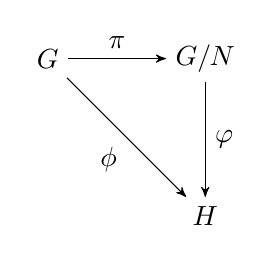
\begin{tikzpicture}[->, >=stealth', node distance=2cm]
    \node (G) {$G$};
    \node[right of=G] (GN) {$G/N$};
    \node[below of=GN] (H) {$H$};
    \draw (G) edge[above] node {$\pi$} (GN)
          (GN) edge[right] node {$\varphi$} (H)
          (G) edge[below left] node {$\phi$} (H);
\end{tikzpicture}
\end{center}

\begin{exercise}
    Prove that if $H$ is a normal subgroup of group $G$ of prime index $p$, then for all $K\leq G$ either $K\leq H$ or $G=HK$ and $|K:K\cap H|=p$.
\end{exercise}

\begin{exercise}
    Let $M$ and $N$ be normal subgroups of $G=MN$. Prove that $(G/M\cap N)\cong (G/M)\times (G/N)$.
\end{exercise}

\begin{exercise}
    Let $G$ be a group of order $p^a m$, where $p$ is a prime that does not divide $m$. Let $P$ be a subgroup of $G$ of order $p^a$ and $N$ a normal subgroup of $G$ of order $p^bn$, where $p$ does not divide $n$. Prove that $|P\cap N|=p^b$ and $|PN/N|=p^{a-b}$. (We shall read about these type of subgroups in detail when we discuss Sylow $p$-subgroups)
\end{exercise}

\begin{exercise}
    A subgroup $H$ of a finite group $G$ is called a \textit{Hall subgroup} of $G$ if $(|G:H|,|H|)=1$. Prove that if $H$ is a Hall subgroup of $G$ and $N\unlhd G$, then $H\cap N$ is a Hall subgroup of $N$ and $HN/N$ is a Hall subgroup of $G/N$.
\end{exercise}

\subsection{Composition Series}

Although proving Cauchy's Theorem was given as an exercise in \ref{exercCauchyThm}, we shall prove the following (weaker) result.

\begin{lemma}
    Let $G$ be a finite abelian group and $p$ be a prime dividing $|G|$. Then $G$ contains an element of order $p$.
\end{lemma}

\begin{definition}
    A non-trivial group $G$ is called \textit{simple} if the only normal subgroups of $G$ are $\{1\}$ and $G$.
\end{definition}

By Lagrange's Theorem, any group of prime order is simple. Also, every abelian simple group is isomorphic to $\mathbb{Z}_p$ for some prime $p$.

\begin{definition}
    Let $G$ be a group. A sequence of subgroups
    $$\{1\}\leq N_0\leq N_1\leq N_2\leq\cdots\leq N_{k-1}\leq N_k=G$$
    is called a \textit{composition series} if $N_i\unlhd N_{i+1}$ and $N_{i+1}/N_i$ is a simple group for each valid $i$. The quotient groups $N_{i+1}/N_i$ are then called \textit{composition factors}.
\end{definition}

\begin{theorem}[Jordan-H\"older]
    Let $G$ be a non-trivial finite group. Then
    \begin{enumerate}[(i)]
        \item $G$ has a composition series and
        \item if $\{1\}=N_0\leq N_1\leq\cdots\leq N_r=G$ and $\{1\}=M_0\leq M_1\leq\cdots\leq M_s=G$ are two composition series of $G$, then $r=s$ and there is some permutation $\pi$ of $\{1,2,\ldots,r\}$ such that
        $M_{\pi(i)}/M_{\pi(i)-1}\cong N_i/N_{i-1}$ for each $1\leq i\leq r$.
    \end{enumerate}
\end{theorem}



\clearpage
\bibliographystyle{plain}
\bibliography{references}
\section*{Acknowledgements}
    I would like to acknowledge \href{https://aryamanmaithani.github.io/}{Aryaman Maithani}'s help in pointing out errors in these notes.
    
    % Note: The converse of Lagrange's Theorem (If $k\in\mathbb{Z}^{+}$ such that $k\mid|G|$, then there exists a subgroup of $G$ of order $k$) holds if $G$ is a finite abelian group.
    
    % To define a homomorphism from a group $G$ to $G'$, it is not enough to define the value of $\varphi$ at the generators of $G$, we must also ensure that the relations are satisfied. That is, if we have a relation $r=1$, where $r$ is some combination of generators, then we must also have that $\varphi (r)=1$.
    
    % Let $H\leq G$. The set of left cosets of $H$ in $G$ is in bijection with the set of right cosets of $H$ in $G$ ($x\mapsto x^{-1}$ maps each left coset to a right coset).
    
    % In a group $G$, a sequence of subgroups $$1=N_{0} \leq N_{1} \leq N_{2} \leq\cdots\leq N_{k-1}\leq N_{k}=G$$ is called a \textit{composition series} if $N_{i} \unlhd N_{i+1}$ and $N_{i+1}/N_{i}$ is a simple group, $0\leq i\leq k-1$. If the above sequence is a composition series, the quotient groups $N_{i+1}/N_{i}$ are called \textit{composition factors} of $G$.
    
    % \textit{Jordan-H{\"o}lder Theorem:} Let $G$ be a finite group with $G\neq 1$. Then
    % \begin{enumerate}[i]
    %     \item $G$ has a composition series.
    %     \item The composition factors in a composition series are unique. Namely, if $1=N_{0} \leq N_{1} \leq N_{2} \leq\cdots\leq N_{r-1}\leq N_{r}=G$ and $1=M_{0} \leq M_{1} \leq M_{2} \leq\cdots\leq M_{s-1}\leq M_{s}=G$, then $r=s$ and there is some permutation $\pi$ of $\{1,2,\cdots, r\}$ such that $M_{\pi(i)}/M_{\pi(i)-1}\cong N_{i}/N_{i-1}$. Note that the series itself need not be unique, but the composition factors are unique.
    % \end{enumerate}    
    
    % \textit{Feit-Thompson}: If $G$ is a simple group of odd order, then $G\cong Z_p$ for some prime $p$.
    
    % A group $G$ is \textit{solvable} if there is a composition series of $G$ such that every composition factor of $G$ is abelian.
    
    % Let $G$ be a finite group. The following are equivalent:
    % \begin{enumerate}[i]
    %     \item $G$ is solvable.
    %     \item $G$ has a composition series such that every composition factor is cyclic.
    %     \item All composition factors of $G$ are of prime order.
    %     \item $G$ has a chain of subgroups: $1=N_{0} \leq N_{1} \leq N_{2} \leq\cdots\leq N_{t-1}\leq N_{t}=G$ such that each $N_i$ is a normal subgroup of $G$ and $N_{i+1}/N_{i}$ is abelian, $0\leq i\leq t-1$.
    %     \item For every divisor $n$ of $|G|$ such that $\left(n,\frac{|G|}{n}\right)=1$, $G$ has a subgroup of order $n$.
    %     \item There exists a normal subgroup $N$ of $G$ such that both $N$ and $G/N$ are solvable.
    % \end{enumerate}
    
    % The permutation $\sigma$ is odd if and only if the number of cycles of even length in its cycle decomposition is odd.
    
    % $A_n$, the alternating group of degree $n$, is a non-abelian simple group for all $n\geq5$.
    
    % An action of $G$ on $A$ may also be viewed as a faithful action of $G/\ker \varphi$ on $A$.

    % Let $G$ be a group acting on a nonempty set $A$. For each $g\in G$, the map $\sigma_{g}:A\to A$ defined by $\sigma_{g}(a)=g\cdot a$ is a permutation of $A$. There is a homomorphism associated with this action of $G$ on $A$ given as $\varphi:G\to S_A$ defined by $\varphi(g)=\sigma_{g}$ called the \textit{permutation representation} associated with this action. The kernel of this action is the same as the kernel of $\varphi$.
    
    % \begin{definition}
    % If $G$ is a group, a \textit{permutation representation} of $G$ is any homomorphism of $G$ into the symmetric group $S_A$ for some nonempty set $A$. We shall say that the given action \textit{affords} or \textit{induces} the associated permutation representation of $G$.
    % \end{definition}
    
    % Let $G$ be a group acting on the nonempty set $A$. The relation on $A$ defined by $a\sim b$ if and only if $a=g\cdot b$ for some $g\in G$ is an equivalence relation. For each $a\in A$, the number of elements in the equivalence class containing $a$ is $|G:G_a|$, where $G_a$ is the stabilizer of $a$.
    
    % Let $G$ be a group, let $H$ be a subgroup of $G$ and let $G$ act by left multiplication on the set $A$ of left cosets of $H$ in $G$. Let $\pi_H$ be the associated permutation representation afforded by this action. Then
    % \begin{enumerate}[i]
    %     \item $G$ acts transitively on $A$.
    %     \item the stabilizer in $G$ of the point $1H\in A$ is the subgroup $H$.
    %     \item the kernel of the action (i.e., the kernel of $\pi_H$) is $\cap_{x\in G}xHx^{-1}$ and $\ker\pi_H$ is the largest normal subgroup of $G$ contained in $H$.
    % \end{enumerate}
    
    % \textit{Cayley's Theorem}: If $G$ is a group of order $n$, then $G$ is isomorphic to a subgroup of $S_n$.
    
    % \textit{Proof}: Just put $H=\{1\}$ in the previous point to get a homomorphism from $G$ to $S_G$. Since the kernel is contained in $H=\{1\}$, $G$ is isomorphic to its image in $S_G$.
    
    % If $G$ is a finite group and $p$ is the smallest prime dividing $|G|$,  any subgroup of index $p$ is normal. Note that, however, a group need not necessarily have a subgroup of index $p$.
    
    % \begin{proof}
    % We have $H\leq G$ and $|G:H|=p$. Let $\pi_H$ be the permutation representation given by multiplication on the set of left cosets of $H$ in $G$. Let $K=\ker \pi_H$ and $|H:K|=k$. Then $|G:K|=|G:H||H:K|$ As there are $p$ left cosets of $H$ in $G$, we have that $G/K$ is isomorphic to a subgroup of $S_p$ (the image of $G$ under $\pi_H$). This implies $pk\mid p!$ and $k\mid (p-1)!$. The minimality of $p$ implies that $|H:K|=1$ and $H=K\unlhd G$.
    % \end{proof}
    
    % Two subsets $S$ and $T$ of $G$ are said to be conjugate in $G$ if there exists $g\in G$ such that $T=gSg^{-1}$.
    
    % The number of conjugates of a subset $S$ of $G$ is the index of the normalizer of $S$, $|G:N_G(S)|$. It follows that the number of conjugates of an element $s$ of $G$ is the index of the centralizer of $s$, $|G:C_G(s)|$. (as $N_G(\{s\})=C_G(s)$)
    
    % \textit{The Class Equation}: Let $G$ be a finite group and let $g_1, g_2, \cdots g_r$ be representatives of the distinct conjugacy classes of $G$ not contained in the center $Z(G)$ of G. Then $$|G|=|Z(G)|+\sum_{i=1}^{r}|G:C_G(g_i)|$$ Note that this is useless for abelian groups.
    
    % If $p$ is a prime and $P$ is a group of prime power order $p^{\alpha}$ for some integer $\alpha\geq 1$, then $P$ has a nontrivial center: $Z(P)\neq \{1\}$.
    
    % \begin{corollary}
    % If $|P|=p^2$ for some prime $p$, then $P$ is abelian. More precisely, $P$ is isomorphic to either $Z_{p^2}$ or $Z_p\times Z_p$.
    % \end{corollary}
    
    % Let $\tau, \sigma$ be members of the symmetric group $S_n$. Then, $\tau\sigma\tau^{-1}$ is obtained from $\sigma$ by replacing each entry $i$ in the cycle decomposition of $\sigma$ with $\tau(i)$.
    
    % If $\sigma\in S_n$ is the product of disjoint cycles of lengths $n_1,n_2,\cdots, n_r$ with $n_1\leq n_2\leq\cdots\leq n_r$ (including its $1$-cycles) then the integers $n_1,n_2,\cdots,n_r$ are called the cycle type of $\sigma$.
    
    % Two elements of $S_n$ are conjugate if and only if they have the same cycle type. The number of conjugacy classes of $S_n$ equals the number of partitions of $n$.
    
    % If $\sigma$ is an $m$-cycle in $S_n$, then $C_{S_n}(\sigma)=\{\sigma^i\tau\mid 0\leq i\leq m-1, \tau\in S_{n-m}\}$ where $S_{n-m}$ denotes the subgroup of $S_n$ which fixes the integers appearing in the $m$-cycle $\sigma$. $|C_{S_{n}}(\sigma)|=m\cdot(n-m)!$.
    
    % If $H\unlhd G$, then for every conjugacy class $\mathcal{K}$ of $G$, either $\mathcal{K}\subseteq H$ or $\mathcal{K}\cap H = \emptyset$.
    
    % If $Z(G)$ is of index $n$, any conjugacy class of $G$ is of order atmost $n$. 
    
    % Assume $H\unlhd G$, $\mathcal{K}$ is a conjugacy class of $G$ contained in $H$ and $x\in\mathcal{K}$. Then, $\mathcal{K}$ is a union of $k$ conjugacy classes of equal size in $H$, where $k = |G\mathrel{:}HC_G(x)|$.
    
    % Let $H\unlhd G$. Then $G$ acts by conjugation on $H$ as automorphisms of $H$. More specifically, the action of $G$ on $H$ by conjugation is defined for each $g\in G$ by $h\mapsto ghg^{-1}$ for each $h\in H$. For each $g\in G$, conjugation by $g$ is an automorphism of $H$. The permutation representation afforded by this action is a homomorphism of $G$ into $\operatorname{Aut}(H)$ with kernel $C_G(H)$. In particular, $G/C_G(H)$ is isomorphic to a subgroup of $\Aut(H)$.
    
    % \begin{corollary}
    % For any $H\leq G$, $N_G(H)/C_G(H)$ is isomorphic to a subgroup of $\Aut(H)$. In particular, putting $H=G$, $G/Z(G)$ is isomorphic to a subgroup of $\Aut(G)$.
    % \end{corollary}
    
    % Let $G$ be a group and $g\in G$. Conjugation by $g$ is called an \textit{inner automorphism} of $G$ and the subgroup of $\Aut(G)$ consisting of all inner automorphisms of $G$ is called $\Inn(G)$. We have that $\Inn(G)\cong G/Z(G)$ and $\Inn(G)\unlhd\Aut(G)$ ($\Aut(G)/\Inn(G)$ is called the outer isomorphism group of $G$)
    
    % $\Aut(Z_n)\cong (\mathbb{Z}/n\mathbb{Z})^{\times}$
    
    % \begin{definition}
    % A subgroup $H$ of $G$ is called \textit{characteristic} in $G$, denoted by $H \operatorname{char} G$, if every automorphism of $G$ maps $H$ to itself, i.e., $\sigma(H)=H$ for all $\sigma\in\Aut(G)$.
    % \end{definition}
    
    % Then,
    % \begin{enumerate}[i]
    %     \item characteristic subgroups are normal,
    %     \item if $H$ is the unique subgroup of $G$ of a given order, then $H \operatorname{char} G$,
    %     \item if $K\operatorname{char} H$ and $H\unlhd G$, then $K\unlhd G$ and
    %     \item if $K\operatorname{char} H$ and $H\operatorname{char} G$, then $K\operatorname{char} G$.
    % \end{enumerate}
    
    % Let $G$ be a group of order $pq$, where $p$ and $q$ are primes (not necessarily distinct) with $p\leq q$. If $p\nmid q-1$, $G$ is cyclic. The proof that $G$ is abelian is as follows.
    
    % \begin{proof}
    % If $Z(G)\neq 1$, then Lagrange's Theorem forces $G/Z(G)$ to be cyclic and hence $G$ to be abelian. Hence we may assume $Z(G)=1$.
    
    % If every nonidentity element of $G$ has order $p$, then the centralizer of every nonidentity element has index $q$, so the class equation for $G$ reads $pq = 1 + kq$. This is impossible since $q$ divides $pq$ and $kq$ but not $1$. Thus $G$ contains an element $x$ of order $q$.
    
    % Let $H=\langle x\rangle$. Since $H$ has index $p$ and $p$ is the smallest prime that divides $|G|$, $H$ is normal in $G$. Since $Z(G)=1$, we must have $C_G(H)=H$. Thus $G/H=N_G(H)/C_G(H)$ is a group of order $p$ isomorphic to a subgroup of $\Aut(H)$. But $\Aut(H)$ has order $\varphi(q)=q-1$ which by Lagrange's Theorem would imply $p\mid q-1$, contrary to the assumption.
    % \end{proof}
    
    % It can further be checked that every such group is cyclic.
    
    % Descriptions of isomorphism types of some automorphism groups:
    
    % \begin{itemize}
    %     \item The automorphism group of the cyclic group of order $p^n$ is cyclic of order $p^{n-1}(p-1)$.
    %     \item For all $n\geq 3$ the automorphism type of the cyclic group of order $2^n$ is isomorphic to $Z_{2}\times Z_{2^{n-2}}$, and in particular is not cyclic but has a cyclic subgroup of index $2$.
    %     \item Let $p$ be a prime and let $V$ be an abelian group (written additively) with the property that $pv=0$ for all $v\in V$. If $|V|=p^n$, then $V$ is an n-dimensional vector space over the field $\mathbb{F}_p=\mathbb{Z}/p\mathbb{Z}$. The automorphisms of $V$ are precisely the nonsingular linear transformations from $V$ to itself, that is, $$\Aut(V)\cong GL(V)\cong GL_n(\mathbb{F}_p).$$ In particular, the order of $\Aut(V)$ is $(p^{n}-1)(p^{n}-p)(p^{n}-p^{2})\cdots(p^n-p^{n-1})$.
    %     \item For all $n\neq 6$ we have $\Aut(S_{n})=\Inn(S_{n})\cong S_{n}$. For $n=6$, we have $|\Aut(S_{6})\mathrel{:}\Inn(S_{6})|=2$.
    %     \item $\Aut(D_8)\cong D_8$ and $\Aut(Q_8)\cong S_4$.
    % \end{itemize}
    
    % \begin{definition}
    % Let $G$ be a group and $p$ be a prime.
    % \begin{itemize}
    %     \item A group of order $p^{\alpha}$ for some $\alpha\geq 1$ is called a \textit{$p$-group}.
    %     \item If $G$ is a group of order $p^{\alpha}m$, where $p\nmid m$, then a subgroup of order $p^{\alpha}$ is called a \textit{Sylow $p$-subgroup} of $G$.
    %     \item The set of Sylow $p$-subgroups will be denote by $Syl_{p}(G)$ and the number of Sylow $p$-subgroups of $G$ will be denoted by $n_{p}(G)$ (or just $n_p$).
    % \end{itemize}
    % \end{definition}
    
    % \textit{Sylow's Theorem}: Let $G$ be a group of order $p^{\alpha}m$ where $p$ is a prime that does not divide $m$.
    % \begin{enumerate}
    %     \item Sylow $p$-subgroups of $G$ exist, i.e., $Syl_p(G)\neq\emptyset$.
    %     \item If $P$ is a Sylow $p$-subgroup of $G$ and $Q$ is any $p$-subgroup of $G$, then there exists $g\in G$ such that $Q\leq gPg^{-1}$, i.e., $Q$ is contained in some conjugate of $P$. In particular, any two Sylow $p$-subgroups of $G$ are conjugate in $G$.
    %     \item The number of Sylow $p$-subgroups of $G$ is of the form $1+kp$, i.e., $$n_p\equiv 1\Mod p.$$ Further, $n_p$ is the index in $G$ of the normalizer $N_G(P)$ for any Sylow $p$-subgroup $P$, hence $$n_p\mid m.$$
    % \end{enumerate}
    
    % Any two Sylow $p$-subgroups of a group (for the same prime $p$) are isomorphic.
    
    % Let $P\in Syl_p(G)$. If $Q$ is any $p$-subgroup of $G$, then $Q\cap N_G(P)=Q\cap P$.
    
    % Let $P$ be a Sylow $p$-subgroup of $G$. Then the following are equivalent:
    % \begin{enumerate}
    %     \item $P$ is the unique Sylow $p$-subgroup of $G$, i.e., $n_p=1$
    %     \item $P\unlhd G$
    %     \item $P\operatorname{char} G$
    %     \item All subgroups generated by elements of $p$-power order are $p$-groups, i.e., if $X$ is any subset of $G$ such that $|x|$ is a power of $p$ for all $x\in X$, then $\langle X\rangle$ is a $p$-group.
    % \end{enumerate}
    
\end{document}
